
\documentclass[a4paper,10pt]{article}
\usepackage{amsmath,amsthm,amssymb,graphicx}

%\usepackage{} %% Please use additional packages only if really necessary.
               %% Make sure that these packages are compatible with amsmath.
\usepackage{enumerate}
\usepackage{enumitem}
\usepackage{float}
\usepackage{tikz}
\usetikzlibrary{graphs,graphs.standard,shapes.geometric,calc}
%\usetikzlibrary{calc}
%\usetikzlibrary{external}
%\tikzexternalize[prefix=figures/]
\usepackage{float}
\usepackage{url}
\usepackage{hyperref}
% Used for pseudocode
\usepackage{algorithm}
\usepackage[noend]{algpseudocode}
\usepackage{caption}

\setlength{\headheight}{0mm}
\setlength{\oddsidemargin}{-0mm}
\setlength{\topmargin}{-15mm}        
\setlength{\textwidth}{160mm}
\setlength{\textheight}{240mm}       
\renewcommand{\baselinestretch}{1.0} 
%\renewcommand{\thefootnote}{\fnsymbol{}}
\renewcommand{\title}[1]{\vspace{\fill}
\eject\addtolength{\baselineskip}{4pt}
{\bfseries\LARGE #1}\\[3mm]\addtolength{\baselineskip}{-4pt}}
\renewcommand{\author}[3]{\parbox[t]{75mm}
{\begin{center}{\scshape #1}\\[3mm] #2\\
 {\ttfamily #3} \end{center}}}

 	
\newcommand{\ml}{${\rm ml}$}
\newcommand{\CZ}[1]{{\color{blue} Carol: #1}}
\newcommand{\WG}[1]{{\color{orange} Gabor: #1}}
\newcommand{\Jarne}[1]{{\color{purple} Jarne: #1}}
\newcommand{\Jan}[1]{{\color{cyan} Jan: #1}}

\newtheorem{thm}{\bfseries Theorem}
\newtheorem{lem}[thm]{\bfseries Lemma}        %% lemmas, props, cor, etc
\newtheorem{remark}[thm]{\bfseries Remark}    %%   are numbered consecutively
\newtheorem{iden}{\bfseries Identity}         %%   with the theorems.
\newtheorem{sublem}{\bfseries Sub-lemma}[thm] %% 
\newtheorem{prop}[thm]{\bfseries Proposition} %%
\newtheorem{cor}[thm]{\bfseries Corollary}     
\newtheorem{defn}[thm]{\bfseries Definition}
\newtheorem{cl}[thm]{\bfseries Claim}
\newtheorem{axiom}[thm]{\bfseries Axiom}
\newtheorem{conj}[thm]{\bfseries Conjecture}
\newtheorem{fact}[thm]{\bfseries Fact}
\newtheorem{hypo}[thm]{\bfseries Hypothesis}
\newtheorem{assum}[thm]{\bfseries Assumption}
\newtheorem{crit}[thm]{\bfseries Criterion}
\newtheorem{exmp}[thm]{\bfseries Example}
\newtheorem{prob}[thm]{\bfseries Problem}
\newtheorem{prin}[thm]{\bfseries Principle}
  
% \newenvironment{proof}{ \medskip                    %% Proof
% \noindent{\scshape Proof:}}{\quad $\Box$\medskip}  %%

%%%%%%%%%%%%%%%%%%%%%%%%%%%%%%
% add below what is needed
%%%%%%%%%%%%%%%%%%%%%%%%%%%%%

%\pagestyle{empty}
\begin{document}

\begin{center}

%%%%%%%%%%%%%%%%%%%%%%%%%%%%%%%%%%%%%%%%%%%%%%%%%%%%%%%%
% Title
%%%%%%%%%%%%%%%%%%%%%%%%%%%%%%%%%%%%%%%%%%%%%%%%%%%%%%%%
\title{Network fault costs based on\\[1mm] minimum leaf spanning trees
 } 
%%%%%%%%%%%%%%%%%%%%%%%%%%%%%%%%%%%%%%%%%%%%%%%%%%%%%%%%
% begin : Authors
%%%%%%%%%%%%%%%%%%%%%%%%%%%%%%%%%%%%%%%%%%%%%%%%%%%%%%%%
\author{Jan Goedgebeur\footnotemark[1]  
%%%%%%%%%%%%%%%%%%%%%%%%%%%%%%%%%%%%%%%%%%%%%%%%%%%%%%%
%%Footnote optional for thanks
%%%%%%%%%%%%%%%%%%%%%%%%%%%%%%%%%%%%%%%%%%%%%%%%%%%%%%
}{
Department of Computer Science\\
KU Leuven Kulak\\
Etienne Sabbelaan 53, 8500 Kortrijk, Belgium \\ and \\ Department of Mathematics, Computer Science and Statistics \\
Ghent University\\
Krijgslaan 281-S9, 9000 Ghent, Belgium
}{
jan.goedgebeur@kuleuven.be
}\footnotetext[1]{Research is supported by Internal Funds of KU Leuven and an FWO grant with grant number G0AGX24N.}
%%%%%%%%%%%%%%%%%%%%%%%%%%%%%%%%%%%%%%%%%%%%%%%%%%%%%
% Add the text of ``thanks'' above
%%%%%%%%%%%%%%%%%%%%%%%%%%%%%%%%%%%%%%%%%%%%%%%%%%%%%
\author{Jarne Renders\footnotemark[1] 
%%%%%%%%%%%%%%%%%%%%%%%%%%%%%%%%%%%%%%%%%%%%
%% Underline the name of the speaker
%%%%%%%%%%%%%%%%%%%%%%%%%%%%%%%%%%%%%%%%%%%
}{Department of Computer Science\\
KU Leuven Kulak\\
Etienne Sabbelaan 53, 8500 Kortrijk, Belgium
}{
jarne.renders@kuleuven.be
}
%
\author{{G\'abor Wiener}\footnotemark[2]
}{ 
Department of Computer Science and Information Theory\\
Budapest University of Technology and Economics\\
M\H uegyetem rkp. 3., 1111 Budapest, Hungary 
}{
wiener@cs.bme.hu
}\footnotetext[2]{Research is supported by project no.\ BME-NVA-02, implemented with the support provided by the Ministry of Innovation and Technology of Hungary from the National Research, Development and Innovation Fund, financed under the TKP2021 funding scheme.}
\author{Carol T. Zamfirescu  
%%%%%%%%%%%%%%%%%%%%%%%%%%%%%%%%%%%%%%%%%%%%%%%%%%%%%%%
%%Footnote optional for thanks
%%%%%%%%%%%%%%%%%%%%%%%%%%%%%%%%%%%%%%%%%%%%%%%%%%%%%%
}{
Department of Mathematics, Computer Science and Statistics \\
Ghent University\\
Krijgslaan 281-S9, 9000 Ghent, Belgium\\ and \\ Department of Mathematics \\ Babe\c{s}-Bolyai University \\ Cluj-Napoca, Roumania
}{
czamfirescu@gmail.com
}%\footnotetext[4]{}


%%%%%%%%%%%%%%%%%%%%%%%%%%%%%%%%%%%%%%%%%%%%%%%%%%%%%%%%
% end : Authors
%%%%%%%%%%%%%%%%%%%%%%%%%%%%%%%%%%%%%%%%%%%%%%%%%%%%%%%%

\end{center}

%%%%%%%%%%%%%%%%%%%%%%%%%%%%%%%%%%%%%%%%%%%%%%%%%%%%%%%%
% Abstract
%%%%%%%%%%%%%%%%%%%%%%%%%%%%%%%%%%%%%%%%%%%%%%%%%%%%%%%%

\begin{quote}
{\bfseries Abstract:}
We study the fault-tolerance of networks from both the structural and computational point of view using the minimum leaf number of the corresponding graph $G$, i.e.\ the minimum number of leaves of the spanning trees of $G$, and its vertex-deleted subgraphs. We investigate networks that are leaf-guaranteed, i.e.\ which satisfy a certain stability condition with respect to minimum leaf numbers and vertex-deletion. Next to this, our main notion is the so-called \emph{fault cost}, which is based on the number of vertices that have different degrees in minimum leaf spanning trees of the network and its vertex-deleted subgraphs. We characterise networks with vanishing fault cost via leaf-guaranteed graphs and describe, for any given network $N$, leaf-guaranteed networks containing $N$. We determine for all non-negative integers $k \le 8$ except 1 the smallest network with fault cost $k$. We also give a detailed treatment of the fault cost 1 case, prove that there are infinitely many 3-regular networks with fault cost 3, and show that for any non-negative integer $k$ there exists a network with fault cost exactly~$k$.
\end{quote}

%%%%%%%%%%%%%%%%%%%%%%%%%%%%%%%%%%%%%%%%%%%%%%%%%%%%%%%%
% Keywords (3 $\sim$ 5 words)
%%%%%%%%%%%%%%%%%%%%%%%%%%%%%%%%%%%%%%%%%%%%%%%%%%%%%%%%
\begin{quote}
{\bf Keywords}: Spanning tree, minimum leaf number, fault cost, hamiltonicity
\end{quote}
\newpage


%%%%%%%%%%%%%%%%%%%%%%%%%%%%%%%%%%%%%%%%%%%%%%%%%%%%%%%%
% Text
%%%%%%%%%%%%%%%%%%%%%%%%%%%%%%%%%%%%%%%%%%%%%%%%%%%%%%%%
\section{Introduction} 
 
We investigate the fault-tolerance of networks using spanning trees of the corresponding graphs. Optimisation problems concerning spanning trees occur in many applications, such as querying in computer database systems and connection routing. Consider a network modelled by a graph $G$. In various applications, in order to minimise costs, it is desirable to describe a spanning tree of $G$ with as few leaves as possible. The number of leaves in such a tree is called the minimum leaf number---the formal definition is given below. This number shall measure the quality of our solution: the smaller the number of leaves in a spanning tree, the better. In this article we want to investigate the situation when, due to a technical failure in the network, one of its nodes becomes unreachable.
We model this by removing the corresponding vertex, which we call $v$, from $G$. In order to achieve a \emph{fault-tolerant} network, we wish to guarantee that the minimum leaf number of $G - v$ is not larger than that of $G$, i.e.\ vertices in $G - v$ remain at least as well reachable as in $G$, and this holds true for an \emph{arbitrary} node of the network as we do not know where the failure will occur. We shall here formalise this idea and give both theoretical as well as computational results.
We will do so from two angles: on the one hand, we will investigate so-called leaf-guaranteed graphs, in which indeed vertices in $G - v$ remain at least as well reachable as in $G$, while on the other hand we shall introduce the notion of \textit{fault cost}, a general tool to gauge how well a given arbitrary network performs with respect to an occurring fault (i.e.,
% \Jarne{Do we use i.e.\ or i.e.,?} \Jan{I have no strong preference as long as we are consistent. Short sidenote afterwards: I see a lot of i.e.\ sentences are part of a very short sentence surrounded by two comma's, so maybe better without the comma to avoid having to add a third comma for very short sentences? Our in principle we could also use i.e.\ for short sentences and i.e., for longer ones (as we did it now, I think)}
in our model, the loss of a node).
% \CZ{I systematically write i.e.\ without a comma thereafter. However, in this case, the i.e.\ is followed by a subordinate clause, namely ``in our model'', hence the comma(s)}


% \Jan{Jarne, in your definition ``For an integer $k \ge 1$, if a graph $G$...'' don't we also need that $G$ is connected?} \Jarne{You are right, I believe we can fix this by defining also $0$-, i.e.\ empty separators. I write for $k\geq 0$ ...} 
%\CZ{I find this less appealing. We could say at the very beginning: A graph is \textit{connected} if there is a path between any two of its vertices. Then we define separators in connected graphs.}
%\Jarne{I have added this below.}
% \Jarne{If you agree please move to a fitting location: For an integer $k \ge 1$, if a graph $G$ has a set of $k$ vertices $X$ for which $G - X$ has at least two connected components, we call $X$ a \emph{$k$-separator} of $G$. $G$ is \emph{$k$-connected} if it has more than $k$ vertices and does not have an $m$-separator for any $m < k$ \CZ{Seems to me we do not capture complete graphs this way (?)... A complete graph on $n \ge 2$ vertices is defined to be $(n-1)$-connected, and a non-complete graph $G$ is \textit{$k$-connected} ... \Jarne{(I think it does capture them. Complete graph on $n$ vertices is not $n$-connected as it does not have more than $n$ vertices, but it is $(n-1)$-connected as it has no $k$-separator $k < n - 1$. We can explicitly state their connectivity but we shuld say " A complete graph on $n \ge 2$ vertices is to be $k$-connected for $1\leq k \leq n-1$")}}, and $G$ is of \emph{connectivity} $k$ if it is $k$-connected and admits a $k$-separator or a set of $k$ vertices whose removal leaves a single vertex.} \CZ{Added below, double-check and remove this when satisfied}
The vertex set and the edge set of a graph $G$ is denoted by $V(G)$ and $E(G)$, respectively. The subgraph of $G$ induced by $X \subseteq V(G)$ is denoted by $G[X]$ and let $G-X := G[V(G)\setminus X]$, $G-v := G-\{ v\}$ for any $v\in V(G)$. For $v,w \in V(G)$ let $G + vw$ denote the graph obtained from $G$ by adding the edge $vw$ to $E(G)$. A graph is \emph{connected} if there is a path between any two of its vertices. For an integer $k \ge 1$, if a connected graph $G$ has a set of $k$ vertices $X$ for which $G - X$ has at least two connected components, we call $X$ a \emph{$k$-separator} of $G$. The graph $G$ is \emph{$k$-connected} if it has more than $k$ vertices and does not have an $m$-separator for any $m < k$, and $G$ is of \emph{connectivity} $k$ if it is $k$-connected and admits a $k$-separator or a set of $k$ vertices whose removal leaves a single vertex. For vertices $v$ and $w$ in a graph, we write \textit{$v$-path} for a path with end-vertex $v$, and \textit{$vw$-path} for a $v$-path with end-vertex $w$. We denote the set of all spanning trees of $G$ as ${\cal T}(G)$. A \textit{leaf} is a vertex of degree~1, and, in a tree, a \textit{branch} is a vertex of degree at least 3. A spanning tree with exactly $k$ leaves is a \textit{$k$-leaf spanning tree}. We call $L(G)$ the set of leaves of a graph $G$ and put $\ell(G) := |L(G)|$. A vertex is \textit{cubic} if it has degree~3, and a graph is \textit{cubic} or \textit{$3$-regular} if all of its vertices are cubic. For a subgraph $H$ of some given graph, if a vertex $v$ in $H$ has exactly $k$ neighbours in $H$, we say that $v$ has \textit{$H$-degree} $k$. Throughout the paper, we assume graphs to be simple, undirected, and 2-connected, unless explicitly stated otherwise.%A graph is \textit{cubic} if all of its vertices have degree 3. \Jarne{cubic graphs defined twice.} OK, the duplicate definition is now removed.

A graph on $n$ vertices is \textit{hamiltonian} if it contains a cycle of length $n$, i.e.\ a \textit{hamiltonian cycle}, and it is \textit{traceable} if it contains a path on $n$ vertices, i.e.\ a \textit{hamiltonian path}. We do not consider $K_1$ or $K_2$ to be hamiltonian. Following~\cite{Wi17}, the \emph{minimum leaf number} ml$(G)$ of a graph $G$ is defined to be 1 if $G$ is hamiltonian, $\infty$ if $G$ is disconnected, and $\min_{T \in {\cal T}(G)} \ell(T)$ otherwise. It is worth pointing out that the minimum leaf number of a graph is bounded above by its independence number, see~\cite[Proposition~8]{GHHSV04}. In a graph $G$, we will call a spanning tree or hamiltonian cycle $S$ with ${\rm ml}(S) = {\rm ml}(G)$ an \emph{ml-subgraph}. For further results on trees with a minimum number of leaves and equivalent problems, we refer to~\cite{GHHSV04,SW08,BFGL13,GOVW19}, and for a pertinent US Patent of Demers and Downing, Oracle Corp., see~\cite{DD00}.

A graph $G$ is \emph{$k$-leaf-guaranteed} if $k = {\rm ml}(G) \ge {\rm ml}(G - v)$ for all $v \in V(G)$. We denote the family of all $k$-leaf-guaranteed graphs with ${\cal L}_k$ and call a graph $G \in \bigcup_k {\cal L}_k$ \emph{leaf-guaranteed}. It is easy to show (but we nonetheless give the proof in the next proposition, for completeness' sake) that $\{{\rm ml}(G - v)\}_{v \in V(G)} \subset \{ k - 1, k \}$ for any $k$-leaf-guaranteed graph $G$.
% \Jarne{$\neq K_2$?} \CZ{We're assuming graphs to be 2-connected; I do wonder whether we should say something about ${\rm ml}(K_1)$, namely that it's 0}.
We write ${\cal L}_k^\ell$ for the set of all graphs $G \in {\cal L}_k$ satisfying ${\rm ml}(G - v) = \ell$ for all $v \in V(G)$, where $\ell \in \{ k - 1, k\}$. Note that ${\cal L}_k \ne {\cal L}_k^k \cup {\cal L}_k^{k-1}$, since there exist graphs of which the vertex-deleted subgraphs  have non-constant minimum leaf number. 

Deciding whether a given graph has a certain minimum leaf number is an NP-complete problem, as it includes the hamiltonian cycle problem as a special case. Leaf-guaranteed graphs offer a common framework for a series of important graph families. ${\cal L}_k^k$ and ${\cal L}_k^{k-1}$ are exactly the \emph{leaf-stable} and \emph{leaf-critical} graphs, respectively, as investigated in~\cite{Wi17}. These generalise hypohamiltonian and hypotraceable graphs and their applications include the solution to a problem of Gargano et al.~\cite{GHHSV04} concerning the wave division multiplexing technology in optical communication. We recall that a graph is \textit{hypohamiltonian} (\textit{hypotraceable}) if the graph itself is non-hamiltonan (non-traceable) yet all of its vertex-deleted subgraphs are hamiltonian (traceable). Hypohamiltonicity---for an overview of theoretical results see the survey of Holton and Sheehan~\cite[Chapter~7]{HS93}---has been applied in operations research in the context of the monotone symmetric traveling salesman problem~\cite{Gr80,GW81} as well as in coding theory~\cite{LMPC12}. Applications related to hypohamiltonicity also appear in the context of designing fault-tolerant networks, see~\cite{LKP05, WHH98}. Moreover, various graph generation algorithms have been designed for hypohamiltonian graphs and related families~\cite{AMW97,GNZ20}. The family ${\cal L}_1^1$ is known as the \emph{$1$-hamiltonian} graphs, a classical notion in hamiltonicity theory~\cite{CKL70}. In applications, these graphs are often called \emph{$1$-vertex fault-tolerant}~\cite[Chapter~12]{HL09}. ${\cal L}_2 \cup {\cal L}_{3}^2$ are exactly the so-called \emph{platypus graphs}~\cite{GNZ20,Za18} which are connected to the Steiner-Deogun property~\cite{KLM96} as described in~\cite{Z}. 

%\Jan{Maybe we should already give a summary of our main results in the introduction and sketch how the rest of the paper is organised?} \CZ{OK} 

In Section~\ref{sec:lgg} we give structural properties of leaf-guaranteed graphs and then prove that for any network~$N$ on $n$ nodes one can describe a leaf-guaranteed network with fewer than $16n$ nodes which contains $N$. In Section~\ref{sec:fc}, the paper's main results are given. These revolve around the notion of a network's \textit{fault cost}. We first give this new notion's formal definition and then give a series of structural results. This is complemented by an algorithm, which we also implemented, to compute the fault cost. For instance, we determine for all non-negative integers $k \le 8$ except 1 the smallest network with fault cost~$k$. We also give a detailed treatment of the difficult fault cost 1 case, prove that there are infinitely many 3-regular networks with fault cost 3, and show that for any non-negative integer $k$ there exists a graph with fault cost exactly $k$. The paper concludes with Section~\ref{sec:probs}, in which we discuss open problems.


\section{Leaf-guaranteed graphs}\label{sec:lgg} 

We begin by summarising some fundamental properties of leaf-guaranteed graphs. %In order to do so we need one more definition. If $G$ is a 2-connected graph and $\{ x, y \}$ a 2-separator in $G$
% \Jan{Should we define $k$-separator?} \CZ{Yes, together with $k$-conn}
%with $G - x - y$ having components $C^1, \ldots, C^k$, then each $G[\{ x, y \} \cup V(C^i)]$ is called a \textit{$2$-fragment of $G$ with attachments $x$ and $y$}.

\begin{prop}\label{prop:lgg} 
Let $G \ne K_2$ be a $k$-leaf-guaranteed graph. Then the following hold.
\begin{enumerate}[label=\normalfont(\roman*)]
\item $G$ is $2$-connected, but not necessarily $3$-connected, and the maximum degree of $G$ is at least~$3$.
\item ${\rm ml}(G - v) \in \{ k-1, k \}$ for all $v \in V(G)$.  %\CZ{Proof has been extended, please have a look.} \Jarne{I agree}
\item For any vertex $v$ in $G$ there exists an ml-subgraph $T$ of $G$ such that $v$ is not a leaf of $T$. Moreover, for every $k$ there exists a $k$-leaf-guaranteed graph $G$ containing a vertex $x$ which is not a leaf in any ml-subgraph of $G$. 
%\item There exists no vertex $v$ such that $G$ contains more than $k$ $2$-fragments with $v$ being an attachment in each such fragment.
\end{enumerate}
\end{prop}

\begin{proof} (i) Assume $G$ has a $1$-separator $\{ x \}$. Then $G - x$ is disconnected, whence ${\rm ml}(G) = \infty$, a contradiction. Every leaf-stable graph and every leaf-critical graph is leaf-guaranteed. Leaf-stable and leaf-critical graphs of connectivity 2 were described in~\cite{OWZ20}, so leaf-guaranteed graphs need not be 3-connected. Since a leaf-guaranteed graph is 2-connected but cycles are not leaf-guaranteed, its maximum degree must be at least~3. 
% \Jarne{Do we need a definition of connectivity $k$ and $k$-connected in intro?} \Jan{I think this would be best, especially as we are not submitting this to a classical graph theory journal.} \CZ{OK}

(ii) Since ${\rm ml}(K_1) = 0$ and ${\rm ml}(K_2) = 2$, the assertion does not hold if $G = K_2$, although $K_2$ is leaf-guaranteed. We now prove the statement for every graph $G \ne K_2$ and assume this henceforth tacitly. We have that ${\rm ml}(G)$ is a positive integer or $\infty$ unless $G = K_1$. As $G$ is leaf-guaranteed we have ${\rm ml}(G - v) \le {\rm ml}(G)$ for any vertex $v$ in $G$ by definition, so the statement holds for all graphs $G$ with ${\rm ml}(G) \le 2$. 

So let ${\rm ml}(G) = k \ge 3$. We continue with a proof by contradiction and suppose ${\rm ml}(G - v) \le k - 2$ for some vertex $v$ in $G$. If there exists a hamiltonian cycle $\mathfrak{h}$ of $G - v$ we can easily modify $\mathfrak{h}$ to a hamiltonian path in $G$, so ${\rm ml}(G) \le 2$, contradicting ${\rm ml}(G) = k \ge 3$. So ${\rm ml}(G - v) \ge 2$ certainly holds for all $v$ in $G$.

Hence we may assume that there exists a spanning tree $T$ of $G - v$ with at most $k - 2 \ge 2$ leaves. Let $w \in N(v)$. Then $\ell(T + vw) \le k - 1$, so ${\rm ml}(G) \le k - 1$, a contradiction. On the other hand, ${\rm ml}(G - v) \ge k + 1$ is impossible, since $G$ is $k$-leaf-guaranteed, so by definition ${\rm ml}(G - v) \le k$.

(iii) Both statements are obviously true for $k = 1$ (as no leaves are present), so assume henceforth $k \ge 2$. In a $k$-leaf-guaranteed graph $G$, consider a spanning tree $T$ with $k$ leaves, one of which shall be $v$. Let $w$ be adjacent to $v$ in $T$ and $u \ne w$ a vertex adjacent to $v$ in $G$ ($u$ exists as $G$ is 2-connected by Proposition~2). Add the edge $uv$ to $T$, resulting in the graph $T'$.

If $u$ is a leaf in $T$, denote by $s$ the vertex adjacent to $u$ in $T$. Removing $us$ from $T'$ we obtain a new spanning tree $T_0$ of $G$. In $T$ as well as $T_0$ the vertex $u$ is a leaf, but $v$ is not a leaf anymore in $T_0$, so $T_0$ certainly does not have more leaves than $T$. In $T_0$ the vertex $s$ must be a leaf, as otherwise $T_0$ would be a spanning tree of $G$ with fewer than $k$ leaves, which is absurd. So $T_0$ is a spanning tree of $G$ with $\ell(T) = \ell(T_0)$ and $v$ is a leaf of $T_0$.

Consider now the situation that $u$ is not a leaf in $T$. Remove from $T'$ the unique edge lying on the unique cycle of $T'$ and incident with $u$ but not $v$. We obtain a new spanning tree $T_1$ of $G$ in which $v$ is not a leaf. Since $\ell(T) = k = {\rm ml}(G)$ the inequality $\ell(T_1) < \ell(T)$ is impossible, so $\ell(T_1) = \ell(T).$ %\Jarne{I believe we might also use this argument when $u$ is a leaf. But fine to leave it like this.}

For the second statement, consider the Petersen graph $P$ and two adjacent vertices $v$ and $w$ in $P$. It is well-known that both $P$ and $P - w$ contain a hamiltonian path with an endpoint in $v$, a property we will refer to as $(\star)$. (The former follows from the fact that $P$ is traceable and vertex-transitive, and the latter from the fact that $P$ is hypohamiltonian.)
% \Jarne{vertex-transitive and hypohamiltonian are not defined, maybe not a problem?} \CZ{I've added def of hypoham, would not add def of vertex-trans}
Consider $k$ pairwise disjoint copies $P^1, \ldots, P^k$ of $P - vw$, denoting the respective copies of $v$ and $w$ in $P^i$ by $v_i$ and $w_i$. We construct a graph $G_k$ by identifying all $v_i$'s, yielding one vertex $x$, and identifying all $w_i$'s, yielding one vertex $y$. We shall see the $P^i$'s as subgraphs of $G_k$.

Let $T$ be a spanning tree of $G_k$. Since $P$ is non-hamiltonian, $T$ contains at least one leaf in each component of $G_k - x - y$. Therefore, ${\rm ml}(G_k) \ge k$. On the other hand, by $(\star)$, the graph $G_k$ contains a spanning tree with exactly $k$ leaves, whence, the minimum leaf number of $G_k$ is precisely $k$. In order to prove that $G_k$ is $k$-leaf-guaranteed, we need to show that ${\rm ml}(G - v) \le k$ for every $v \in V(G_k)$. We need to differentiate between two cases. If $v \in \{ x, y \}$, then we make use of $(\star)$ and obtain the desired conclusion. If $v \notin \{ x, y \}$, then there exists an $i \in \{ 1, \ldots, k \}$ such that $v \in V(P^i)$. Since $P$ is hypohamiltonian, there exists a hamiltonian $x$-path in $P^i - v$. Combining this with $(\star)$, we obtain a spanning tree of $G_k - v$ with exactly $k$ leaves. Thus, $G_k$ is $k$-leaf-guaranteed. To conclude the proof, we will show that there exists no spanning tree $T$ in $G_k$ which has $k$ leaves, and one of the leaves of $T$ is $x$. However, as noted above, $T$ contains at least one leaf in each component of $G_k - x - y$, of which there are $k$ by construction. Therefore, $T$ has at least $k + 1$ leaves, a contradiction. \end{proof}

%(iv) Let ${\cal F}$ be the set of all 2-fragments in $G$ having $v$ as an attachment. Suppose $|{\cal F}| \ge k+1$. A spanning tree $T$ in $G - v$ must contain at least one leaf in each element of ${\cal F}$, whence $\ell(T) \ge k+1$. But this contradicts the fact that $G$ is $k$-leaf-guaranteed. \Jarne{I do not seem to see this anymore, do the elements in $\mathcal{F}$ have disjoint vertex sets, if not why do the leaves need to be different?} \CZ{The elements in $\mathcal{F}$ have pairwise disjoint interior, where their interior is defined as the whole thing minus attachments} \Jarne{I am not sure I understand. Taking $G$ for example to be the right graph of Fig. 8. It is two leaf stable, let $v = z$ and call the vertex north of $z$ $u$. Then there are two fragments given by the separator $\{z,u\}$ and two by the separator $\{z,w\}$, no? These do not have disjoint interiors, but I might be misunderstanding something.} \CZ{You are right. I propose removing this} \Jarne{OK, I do not think we use it anywhere.}



It is natural to ask whether, given a network $N$, we can find a larger network $N'$ containing a copy of $N$ (or, in graph-theoretical terms: $N$ is an induced subgraph of $N'$) such that $N'$ is leaf-guaranteed. It is known that this is possible if $N'$ may be 40 times larger than $N$: in~\cite{ZZ18} it was shown that any graph $G$ of order at most $n$, connected or not, occurs as induced subgraph of some hypohamiltonian and thus 2-leaf-guaranteed graph of order $40n$. Relaxing the conditions and only requiring containment in a leaf-guaranteed graph, we can describe significantly smaller solutions.

\begin{thm} \label{thm:ind-subgr}
Let $G \ne K_1$ be a possibly disconnected graph of order $n$ containing a longest path~$\mathfrak{p}$ which has $p$ vertices. Put $k := 2n - p + 1$. Then $G$ occurs as an induced subgraph of some $1$-leaf-guaranteed graph of order $k + 1$ as well as of a $k$-leaf-guaranteed graph of order 
$8k$.
% $9k$. 
\end{thm}

\begin{proof} Consider a $k$-cycle $C = v_1 \ldots v_k$ disjoint from $G$. Put $\mathfrak{p} = w_1 \ldots w_p$ and $V(G) \setminus V(\mathfrak{p}) = \{ w_{p+1}, \ldots, w_n \}$. Identify $v_i$ with $w_i$ for all $i \in \{ 1, \ldots, p \}$ and $v_{p + 2j}$ with $w_{p+j}$ for all $j \in \{ 1, \ldots, n-p \}$. We have produced a graph $H$, where the purpose of the identification we just performed is to guarantee that $G$ is indeed an induced subgraph of $H$.

For the first part of the statement, consider the graph $H'$ of order $2n - p + 2 = k + 1$ obtained by taking $H$ and an additional vertex $v_0$, and joining by an edge $v_0$ to $v_i$ for all $i \in \{ 1, \ldots, k \}$. That $H'$ is 1-leaf-guaranteed is easy to see: Considering $C$ now as a subgraph of $H'$, we can replace the edge $v_1v_2$, which lies in $C$, by the path $v_1v_0v_2$ to obtain a hamiltonian cycle in $H'$. The cycle $C$ itself is a hamiltonian cycle in $H' - v_0$. Consider $v$, an arbitrary vertex in $H' - v_0$, and let $u$ and $w$ be $v$'s neighbours on $C$. Adding to the $uw$-path $C - v$ the path $uv_0w$ yields a hamiltonian cycle in $H' - v$. Finally, it is clear that $G$ is an induced subgraph of $H'$, so the first part of the theorem is proven.

Let $\Xi_8$ be the 8-vertex graph obtained by connecting two vertices by three edges, subdividing once any two of the three edges, and blowing up the two cubic vertices to triangles (see the right-hand side of Fig.~\ref{fig:replace_with_Xi_8}). For the theorem's second statement, replace in $H$ every edge of $C$ by a copy of $\Xi_8$, see Fig.~\ref{fig:replace_with_Xi_8}. We now show that the resulting graph $H''$ is $k$-leaf-guaranteed. Let $S \in {\cal S}_{{\rm ml}}(H'')$. It is easy to check that $\Xi_8$ contains no hamiltonian $vw$-path, where $v$ and $w$ are vertices as shown in Fig.~\ref{fig:replace_with_Xi_8}. Thus $S$ must contain at least one leaf in each copy of $\Xi_8$ present in $H''$, whence $\ell(S) \ge k$.

\begin{figure}[!htb]
    \centering
    \begin{tikzpicture}[fo/.style={draw, circle, fill=black, minimum size={0.15cm}, inner sep=0cm, scale=0.65}, scale=0.4]
        \node[fo] (v) at (0,0) {};
        \node[fo] (w) at (8,0) {};
        \node[] (v') at (-3,-1) {};
        \node[] (w') at (11,-1) {};
        \draw (v) -- (w);
        \draw (v) -- (v');
        \draw (w) -- (w');
    \end{tikzpicture}
    \begin{tikzpicture}[scale=0.4]
        \node[scale=1.5] at (0,2) {$\longrightarrow$};
        
        % Invisible nodes giving same height as left and right tikzpictures
        \node[fill=white] at (0,-1) {}; 
        \node[fill=white] at (0,4) {};
    \end{tikzpicture}
    \begin{tikzpicture}[fo/.style={draw, circle, fill=black, minimum size={0.15cm}, inner sep=0cm, scale=0.65}, scale=0.4]
        \node[fo, label=below:$v$] (v) at (0,0) {};
        \node[fo] (1) at (0,4) {};
        \node[fo] (2) at (2,2) {};
        \node[fo, label=below:$w$] (w) at (8,0) {};
        \node[fo] (3) at (8,4) {};
        \node[fo] (4) at (6,2) {};
        \node[fo] (5) at (4,4) {};
        \node[fo] (6) at (4,2) {};
        \node[] (v') at (-3,-1) {};
        \node[] (w') at (11,-1) {};
        \draw (v) -- (w);
        \draw (v) -- (v');
        \draw (w) -- (w');
        \draw (v) -- (1) -- (2) -- (v);
        \draw (w) -- (3) -- (4) -- (w);
        \draw (1) -- (5) -- (3);
        \draw (2) -- (6) -- (4);
    \end{tikzpicture}
    \caption{Replacing an edge with a copy of the graph $\Xi_8$.}
    \label{fig:replace_with_Xi_8}
\end{figure}

It is straightforward to construct a tree with exactly $k$ leaves in $H''$, so $\mathrm{ml}(H'') = k$. It remains to prove that $\mathrm{ml}(H'' - v)\le k$ for every $v \in V(H'')$. By construction, we can restrict ourselves to an arbitrary but fixed copy of $\Xi_8$ in $H''$. It is easy to check that for every vertex $u$ in $\Xi_8$, there exists a hamiltonian path in $\Xi_8 - u$ with at least one endpoint in $V(\Xi_8)\cap V(C)$; see Fig.~\ref{fig:Xi_8_K1-traceable} in Appendix~\ref{app:figure_proof_thm2}. As before, we can complete this path to a spanning tree of $H'' - u$ with exactly $2k$ leaves. We have proven that ${\rm ml}(H'' - v) \le k$ for every vertex $v$ in $H''$, whence, $H''$ is $k$-leaf-guaranteed.
\end{proof}
% \hfill $\Box$

%% OLD PROOF WITH Xi_9

% Let $\Xi$ be the 9-vertex graph obtained by connecting two vertices by three edges, subdividing each edge once, and blowing up the two cubic vertices to triangles (see the right-hand side of Fig.~\ref{fig:ind-subgr1}). We remark that $\Xi$ is the smallest 2-leaf-guaranteed graph in terms of order, and among 9-vertex graphs it has the smallest size; there are three others on $9$ vertices obtained from $\Xi$ by adding one, two, and three edges respectively.

% For the theorem's second statement, replace in $H$ every edge of $C$ by a copy of $\Xi$, see Fig.~\ref{fig:ind-subgr1}. We now show that the resulting graph $H''$ is $k$-leaf-guaranteed. Let $S \in {\cal S}_{{\rm ml}(H'')}$. It is easy to check that $\Xi$ contains no hamiltonian $vw$-path. Thus $S$ must contain at least one leaf in each copy of $\Xi$ present in $H''$, whence $\ell(S) \ge k$.

% \begin{figure}[h]
% \begin{center}
% \includegraphics[height=20mm]{lg-fig2}\\
% \caption{Replacing an edge with a copy of the graph $\Xi$.}\label{fig:ind-subgr1}
% \end{center}
% \end{figure}

% It is straightforward to construct a tree with exactly $k$ leaves in $H''$, so ${\rm ml}(H'') = k$. It remains to prove that ${\rm ml}(H'' - v) \le k$ for every $v \in V(H'')$. By construction, we can restrict ourselves to an arbitrary but fixed copy of $\Xi$ in $H''$. Fig.~\ref{fig:ind-subgr2} shows that for every vertex $u$ in $\Xi$, there exists a hamiltonian path in $\Xi - u$ with at least one endpoint in $V(\Xi) \cap V(C)$.

% \begin{figure}[h]
% \begin{center}
% \includegraphics[height=55mm]{lg-fig3}\\
% \caption{Hamiltonian paths in vertex-deleted subgraphs of $\Xi$ required to show that ${\rm ml}(H'' - v) \le k$ for every $v \in V(H'')$.}\label{fig:ind-subgr2}
% \end{center}
% \end{figure}

% As before, we can complete this path to a spanning tree of $H'' - u$ with exactly $2k$ leaves. We have proven that ${\rm ml}(H'' - v) \le k$ for every vertex $v$ in $H''$, whence, $H''$ is $k$-leaf-guaranteed. \hfill $\Box$


%\CZ{Of course it would be nice to improve the coefficient (9) here} 
% \Jarne{I think it can be done by smoothing the middle vertex. There is still no hamiltonian $vw$-path \CZ{@Jarne, please have a look: I understand the smoothing as replacing one of the horizontal 3-vertex paths by an edge, but then there IS a ham $vw$-path, so you must mean something else; please explain} and deleting any vertex still has a hamiltonian $v$ or $w$-path. A small computer check seems to indicate this is the smallest graph with these properties.} \Jarne{@Carol: I was a bit imprecise, your definition of smoothing is indeed the same as mine. However, after smoothing we should take $v$ and $w$ to be the endpoints of the new edge.}
%\CZ{I see. Can you write the $8k$ proof?} \Jarne{Done. However, we still refer in the Appendix to $\Xi$ from the old proof. I will let someone else adapt this.}

%\subsection{On a question of Gr\"otschel}

We end this section with a brief remark regarding a question of Gr\"otschel. He asked in~\cite[Problem 4.56]{GGL95} whether \textit{bipartite} hypotraceable graphs exist, i.e.\ whether any member of ${\cal L}_3^2$ is bipartite; note that hypohamiltonian graphs, i.e.\ members of ${\cal L}_2^1$, cannot be bipartite. As there has been little progress on this question, we relax it and ask for bipartite leaf-guaranteed graphs. 
In the upcoming Section~\ref{sec:computation} we describe an algorithm to determine the fault cost of a graph, a notion we shall define later. For a given graph $G$ it computes ml-subgraphs of $G$ and $G - v$ for all $v\in V(G)$. A straightforward adaptation allows to verify whether a graph is leaf-guaranteed. We generate $2$-connected bipartite graphs using \texttt{geng}~\cite{MP14} and then apply our program~\cite{GRWZ25} to check whether the input graphs are $k$-leaf-guaranteed for a certain $k$.
% \Jan{Maybe better: and then apply our algorithm from Section~\ref{sec:computation} whose implementation can be found in~\cite{GRWZ25}?} \Jarne{We only describe the fault cost algorithm in~\ref{sec:computation}, but no algorithm for checking leaf-guaranteed graphs. However, the adaptation should be straightforward and the reader can find the code for checking leaf-guaranteed at~\cite{GRWZ25}} \Jan{Ok, thanks for the clarification. Then better leave it as is with ``our program''.}.
Our computations yield that up to order $15$, there is exactly one $2$-connected bipartite leaf-guaranteed graph
% \footnote{See \url{https://houseofgraphs.org/graphs/53086}.}
of order $12$ (see Fig.~\ref{fig:bip_leaf_guar}) and 
% . It is $2$-leaf-stable, i.e.\ a member of ${\cal L}_2^2$ 
five more $2$-connected bipartite leaf-guaranteed graphs on order $14$. Restricting to girth at least $6$ up to order 22 there is this aforementioned graph on order $12$ as well as six more leaf-guaranteed graphs on order 16; $27$ on order 18; $815$ on order 20; and 11\,775 on order 22.
% \Jan{Possibly remove the footnote to the HoG link if you wish and instead we could add a Figure of the smallest one. \CZ{Yes, that would be better perhaps} For the larger graphs you could write something like: ... can be obtained from the database of interesting graphs at the \textit{House of Graphs}~\cite{CDG23} by searching for the keywords ``XYZ''.} \Jarne{Which should I put on there? All is not possible.} \Jan{Aha, I didn't know there were that many. Then maybe just drop the reference to HoG and let's see if the referees ask about it or not. Possibly you could also consider to make a figure of the 5 graphs of order 14 if they are interesting enough (but I think just the one graph will probably be fine).} 
%\CZ{Yes, I also think one graph is fine. I also wouldn't make too many statements regarding their number when the numbers get so large... it suffices to say that there are (at least) thousands when going beyond a certain order} \Jarne{Fine like this or do you want to reformulate it to remove some of the exact numbers?}
All of them are $2$-leaf-guaranteed bipartite graphs and hence are $2$-leaf-stable, i.e.\ in $\mathcal{L}_2^2$. We did not find any $k$-leaf-guaranteed examples with $k > 2$.
% All examples found were $2$-leaf-stable, i.e.\ members of ${\cal L}_2^2$. We did not find any $k$-leaf-guaranteed examples with $k > 2$.

% \Jarne{Do you see some reason why these examples do not occur on odd orders?} \CZ{Vertex-del subgr of odd-order bip gr cannot be traceable; or do you mean something else?} \Jarne{I see now. We even have that all $2$-leaf-guaranteed bipartite graphs are $2$-leaf-stable, right? \CZ{I think you're right} So my comment above does not make much sense. Maybe we should say: Note that all $2$-leaf-guaranteed bipartite graphs are $2$-leaf-stable, i.e.\ in $\mathcal{L}_2^2$. We did not find any $k$-leaf-guaranteed examples with $k > 2$.} \CZ{OK, but without the 'Note that'}

\begin{figure}[!htb]
    \centering
    \newcommand{\s}{8}
    \begin{tikzpicture}[transform shape, scale=1.5, rotate=-45]
        \tikzstyle{fo} = [draw, circle, fill=black, minimum size={0.15cm}, inner sep=0cm, scale=0.65]
        
        \node[draw=black,minimum size=2cm,regular polygon,regular polygon sides=\s] (a) {};
        
        \foreach \x in {1,2,...,\s}
        	\node[fo] (a\x) at (a.corner \x) {}; 
        \foreach \x in {1,2,...,\the\numexpr\s/2\relax} {
        	\draw (a\x) to (a\the\numexpr\x+\s/2\relax); 
            \node (b) at (a\the\numexpr\x+\s/2\relax) {};
            \node[fo] at ($(a\x)!0.3!(b)$) {};
        }
        % \draw (a\the\numexpr\s\relax) to (a1);
    \end{tikzpicture}
    \caption{The smallest bipartite leaf-guaranteed graph.}
    \label{fig:bip_leaf_guar}
\end{figure}

\section{Fault cost}\label{sec:fc}

\subsection{Definition}

We now introduce the notion of fault cost. From an application-oriented perspective it is important to point out that when a node drops from the network, the ml-subgraph used in the fault-free network may require changing equipment\footnote{We see vertices of different degrees as requiring different equipment in the network. As Salamon and Wiener write in~\cite{SW08}, various problems related to ours have an objective function that depends on the vertex degrees of the spanning tree, see for instance~\cite{GHHSV04,LR98,So98}. This model is particularly useful when designing networks where device costs depend on the required routing functionality.} in many nodes in order to obtain an ml-subgraph in the faulty network, which is undesirable. We formalise this by introducing, for a spanning tree or hamiltonian cycle $S$ of $G$ and a spanning tree or hamiltonian cycle $S_v$ of $G - v$, the \emph{transition cost from $S$ to $S_v$} as
$$\tau(S,S_v) := |\{ w \in V(G) \setminus \{ v \} : \deg_S(w) \ne \deg_{S_v}(w) \}|.$$
Thus, this is the number of vertices in $G$ which need to receive different equipment after the loss of a node; the lost node is ignored in this process. For a given graph $G$, denote by ${\cal S}_{{\rm ml}}(G)$ the set of all of its ml-subgraphs. In order to quantify the optimal solution in a worst-case scenario for the network itself, we introduce for a given graph $G$ and an ml-subgraph $S$ of $G$ the quantity
$$\varphi_S(G) := \max_{v \in V(G)} \min_{S_v \in {\cal S}_{{\rm ml}}(G - v)} \tau(S,S_v).$$
Based on this, we shall consider the \emph{fault cost} $\varphi(G)$ of the graph $G$ representing the network:
$$\varphi(G) := \min_{S \in {\cal S}_{{\rm ml}}(G)} \varphi_S(G).$$

We give an example of how these definitions work in Appendix~\ref{app:fc2_example}. This framework is motivated by the fact that in a practical application one knows the network but must choose one of the ml-subgraphs without knowing which node might
fail---so a subgraph ought to be chosen which minimises the maximum transition cost. We
shall call such a subgraph, i.e.\ an ml-subgraph $S$ in $G$ satisfying $\varphi_{S}(G) = \varphi(G)$, \textit{optimal}.
Finally, when a vertex does fail, one again has the freedom to choose an ml-subgraph (in the
faulty network) bearing the lowest transition costs\footnote{In this model, it may happen that for a certain ml-subgraph only a few nodes are responsible for a high transition cost (and all other nodes yield far lower transition costs), but that for another ml-subgraph the transition costs are more evenly distributed and on average worse, but that the worst-case transition cost is in fact lower, so this latter tree will be chosen. This may not be desirable in certain applications, in particular when nodes fail with varying probabilities. However, in this article we are interested in conserving (or decreasing) the minimum leaf number whenever \emph{any} vertex fails, irrespective of failure probability.}.

\subsection{Computational approach}\label{sec:computation}

%\Jan{I added two subsubsections to make this very long subsection more structured. Feel free to undo this if you don't like it.}

\subsubsection{An algorithm for computing the fault cost}
\label{subsect:algo}

Henceforth we focus on the description, both structural as well as computational, of graphs with small fault cost. For the latter approach we designed an algorithm to computationally determine the fault cost of a given graph.
% It uses backtracking to store the distinct degree sequences of all ml-subgraphs of the given graphs and its vertex-deleted subgraphs \Jan{This sentence sounds a bit strange to me. Normally you store things in a data structure, which backtracking of course isn't. Maybe better something like: We use a backtracking approach and efficiently compute and store the distinct degree sequences using bitsets...?}.
We use a backtracking approach and efficiently compute and store the distinct degree sequences of all ml-subgraphs and its vertex-deleted subgraphs.
Once they have been determined, the degree sequences are compared and the fault cost determined. We use pruning rules, explained in more detail later in this section, in several places to speed up the computations. Our implementation of the algorithm is open source and can be found on GitHub~\cite{GRWZ25}. An overview of the algorithm can be found in Algorithm~\ref{alg:fc}. %\CZ{@Jarne: Seems to me that for any graph $G$, in any ml-subgraph $S$ of $G$, no two leaves of $S$ are adjacent. Is this useful for your alg?} \Jarne{Sadly no, as we construct tree by adding edges, the leaves might change, so we cannot prune yet if they are adjacent. I tried checking for adjacent leaves once a spanning tree is found as we can immediately drop the best found minimum leaf number by one, but it does not seem worth the overhead.}

\begin{algorithm}[!htb]
\caption{computeFaultCost($G$)}\label{alg:fc}
\begin{algorithmic}
    \If{$G$ is $1$-hamiltonian}
        \State \Return 0
    \EndIf
    \State generateAndStoreMinLeafDegreeSequences($G$) // Algorithm~\ref{alg:findMLSequences}
    % \State \Jan{In this font the MlD looks a bit strange as the l resembles a 1. Perhaps just write generateAndStoreMinLeafDegreeSequences (it's longer but it still fits on the page)?}
    \For{$v\in V(G)$}
        \State generateAndStoreMinLeafDegreeSequences($G - v$)// Algorithm~\ref{alg:findMLSequences}
    \EndFor
    \For{Sequence $L$ of $G$}
        \For{$v\in V(G)$}
            \For{Sequence $L_v$ of $G - v$}
                \State Compute transition cost
            \EndFor
            \State Store minimum transition cost over $L_v$'s
        \EndFor
        \State Store maximum of minimum transition costs over $v$'s
    \EndFor
    \State \Return $\varphi(G)$
\end{algorithmic}
\end{algorithm}



In more detail our algorithm works as follows. 
% \Jan{I think it would also be helpful for the reader to give a rough pseudocode of the complete algorithm.} \Jarne{See Algorithm~\ref{alg:fc}} \Jan{Sounds good, thanks!}
Given an input graph $G$, we first check whether it is $1$-hamiltonian using a program~\cite{GRWZ22} designed by the authors for~\cite{GRWZ24}. If the graph is $1$-hamiltonian---clearly, there are infinitely many such graphs---, then we know by the following proposition that its fault cost is~$0$.

\begin{prop}\label{fc0}
A graph has fault cost $0$ if and only if it is $1$-hamiltonian, i.e.\ $1$-leaf-guaranteed.
\end{prop}
\begin{proof} Recall that we work under the general assumption that our graphs are 2-connected, hence we do not treat $K_2$ (which is 1-leaf-guaranteed but not 1-hamiltonian). It is clear that a 1-hamiltonian graph $G$ satisfies $\varphi(G) = 0$, so let us now assume that there exists a non-1-hamiltonian graph $G$ with $\varphi(G) = 0$. The graph $G$ cannot be hamiltonian, for otherwise there would exist a vertex $x$ in $G$ such that $G - x$ is non-hamiltonian. Thus, any ml-subgraph of $G-x$ would have at least two leaves, in which case the fault cost of $G$ would be at least 2, a contradiction. Therefore $G$ is non-hamiltonian and all of its vertex-deleted subgraphs must also be non-hamiltonian, similarly to the previous situation. Let now $T$ be an optimal ml-subgraph of $G$. By the above arguments, $T$ must be a tree. Consider a leaf $b$ of $T$ and let $T_b$ be an arbitrary ml-subgraph of $G - b$. Again, by the above, $T_b$ must be a tree. Then $\varphi(G) = 0$ implies 
$$\tau(T,T_b) = |\{ v \in V(G) \setminus \{ b \} : \deg_T(v) \ne \deg_{T_b}(v) \}| = 0,$$
so
$$\sum_{v \in V(G)} \deg_T(v) = \deg_T(b) + \sum_{v \in V(G) \setminus \{ b \}} \deg_{T_b}(v),$$
which, if we set $n := |V(G)|$, is equivalent to $2(n - 1) = 1+ 2(n-2),$ a contradiction. 
\end{proof}

%Before resuming the description of our program, we apply Proposition~\ref{fc0} to show that in leaf-guaranteed graphs we can give the following upper bound for their fault cost. 

%\begin{prop}
%Every $k$-leaf-guaranteed graph $G$ satisfies $\varphi(G) \le 2k$. \CZ{Double-check Prop 4; it's really not a big deal, but it connects---if it's correct---leaf-guaranteed graphs and fault cost better than anything else we have}
%\end{prop}

%\begin{proof} 
%By Proposition~\ref{fc0}, every 1-leaf-guaranteed graph satisfies $\varphi(G) = 0$, so we may assume henceforth that $k \ge 2$; in particular, we may assume that any ml-subgraph of $G$ is a tree. We have ${\rm ml}(G) = k$, so there exists an optimal tree $S$ in $G$ with $k$ leaves. Let $v \in V(G)$ be an arbitrary vertex and $S_v$ an ml-subgraph in $G - v$.

%First, we consider the case that $S_v$ is a hamiltonian cycle in $G - v$. Then $S$ must be a hamiltonian path, so ${\rm ml}(G) = 2$. Hence $\varphi(G) = 2$. If $S_v$ is not a hamiltonian cycle in $G - v$, then $S_v$ is a tree spanning $G - v$. Then, by Proposition~\ref{prop:lgg}~(ii), $S_v$ has either $k-1$ or $k$ leaves. If $L(S) \cap L(S_v) = \emptyset$ (where we see $S_v$ as a subgraph of $G$), then \Jarne{at most?, e.g., when $v$ is a leaf} $2k$ entries of the degree sequences of $S$ and $S_v$ differ---more is impossible. \Jarne{I am not sure, can't the branches also change degree?} \CZ{Of course. Result is ancient, so probably uses an old def of fc. I don't see how we can fix this. Does anybody else? If not, we remove this.} So we have that $\tau(S,S_v) \le 2k$, from which the statement follows. \end{proof}

We now continue with the description of our algorithm. If $G$ is not $1$-hamiltonian, we will determine all distinct degree sequences of all its ml-subgraphs (see Algorithm~\ref{alg:findMLSequences}). 

\begin{algorithm}[!htb]
\caption{generateAndStoreMinLeafDegreeSequences($G$)}\label{alg:findMLSequences}
\begin{algorithmic}
    \State Create $\mathcal{L}$ // Data structure for storing the sequences
    \If{$G$ is hamiltonian} // Already known if we computed $1$-hamiltonicity
        \State Store single sequence $L$ where all degrees are $2$
        \State \Return $\mathcal{L}$
    \EndIf
    \For{each non-edge $uv$ of $G$}
        \If{$G$ has hamiltonian $uv$-path}
            \State Store sequence $L$, where $u$, $v$ have degree $1$ and $x\neq u,v$ has degree $2$
        \EndIf
    \EndFor
    \If{$\mathcal{L}$ is not empty} // $G$ is traceable
    % \Jan{Ik ga ervan uit dat je in de praktijk test of $\mathcal{L}$ niet leeg is ipv nog eens de traceerbaarheid te testen? Misschien daarom beter schrijven if ($\mathcal{L}$ is not empty) return // Comment: $G$ is traceable?} WG: Szuper volt valamit flamandul is olvasni benne (bár elég keveset értettem belőle...)!
        \State \Return $\mathcal{L}$
    \EndIf
    \For{each ml-subgraph of $G$} // Determined via backtracking and using pruning rules
        \State Compute degree sequence $L$
        \If{$L\not\in\mathcal{L}$}
            \State Store $L$ in $\mathcal{L}$
        \EndIf
    \EndFor
    \State \Return $\mathcal{L}$
    
\end{algorithmic}    
\end{algorithm}

If the graph is hamiltonian (which we do not need to check again), its ml-subgraphs are the hamiltonian cycles of the graph. However, in that case there is only one distinct degree sequence, namely, the one in which every vertex has degree $2$. If the graph is not hamiltonian, using methods from~\cite{GRWZ22}, we determine for every pair of non-adjacent vertices, whether or not there is a hamiltonian path between them. As the graph is not hamiltonian, there cannot be a hamiltonian path between adjacent vertices. For every non-adjacent pair we only need to determine one hamiltonian path as for every such hamiltonian path the degrees of every vertex except for the leaves are $2$ and hence the degree sequences are the same. If we did not find any hamiltonian path in the graph, then we perform an exhaustive search for all ml-subgraphs as follows. 

Using a backtracking algorithm, we generate all spanning trees of the graph. We start with one vertex and every iteration, we choose an edge incident to the current subtree which is not forbidden and first add it to the subtree (if it does not create a cycle), while later we forbid the edge. We then do the same for this newly acquired subtree or newly acquired set of forbidden edges. For the efficiency of the algorithm, we choose an edge for which the endpoint in the subtree $v$ is most constrained.
% meaning the difference between the degree of $v$ in $G$ with the sum of the degrees of $v$ in the subtree and in the graph induced by all forbidden edges is minimal
This means that, denoting the subtree by $T$ and the subgraph of $G$ induced by the forbidden edges by $F$, we want $d_G(v) - d_T(v) - d_F(v)$ to be minimal.
% \Jan{I found this long sentence pretty hard to read, but unfortunately I don't really see a better way to phrase it...} \Jarne{Changed it to be more precise.}
Its other endpoint is the neighbour of $v$ which is most constrained in the same way, such that the edge is not forbidden and not yet in the tree. We can backtrack whenever a vertex of $G$ not yet in the tree is only incident with forbidden edges.

If the tree has size $\lvert V(G)\rvert -1$, we have a spanning tree of our graph. If it has the same number of leaves as the minimum encountered so far, we store its degree sequence in a list. If it is smaller than the minimum encountered so far, we clear the list, store this degree sequence as its first entry and keep track of this new minimum. Since we know the minimum encountered so far, we can actually prune the search as soon as the subtree has more leaves than this minimum. Due to the way we generate the spanning trees, the number of leaves can never decrease unless we backtrack.

In this way, we obtain all ml-subgraphs of $G$ and we repeat this procedure for every vertex-deleted subgraph $G-v$. However, if $v$ was a leaf of an ml-subgraph of $G$, we already know that ${\rm ml}(G)$ is an upper bound for the minimum leaf number of $G -v$ and keep track of this in order to prune earlier. 

Now that we have every distinct degree sequence, we need to compare each degree sequence of the graph with each degree sequence of the vertex-deleted subgraphs. We also use some 
% unsophisticated but 
impactful techniques 
% \CZ{@Jarne: changed from 'tricks'; choice of words OK?} \Jan{Sounds good to me.} 
%\Jarne{Removed "unsophisticated".}
to speed up these
% \Jan{maybe better: these computations?} 
computations. For every degree sequence of an ml-subgraph of $G$, we compare it to the distinct degree sequence of a vertex-deleted subgraph in order to determine the minimum transition cost. While checking the transition cost for two degree sequences is linear in the number of vertices, we also keep track of the leaves and degree $2$ vertices of the graph, by means of bitsets.
These low degree vertices can then be compared in constant time and we only need to iterate over the vertices of degree at least $3$, i.e.\ the branches, in the ml-subgraphs. As the number of branches is relatively small (for example of the 153\,620\,333\,545 graphs of order $12$  which are $2$-connected, only 144 of their ml-subgraphs contained four branches, while none contained more than four), the gain from this method outweighs the overhead of creating the extra bitsets and storing the degree $2$ vertices in terms of efficiency. We also apply a small optimisation
% \CZ{To my surprise this word does seem to exist in some EN dictionaries, but I still recommend 'optimisation'} 
when iterating over the vertices. When the transition cost is already higher than one found earlier, we need not iterate over the remaining vertices. The minimum transition cost is then compared to those of other vertex-deleted subgraphs to determine the maximum. Finally, the minimum of these values is determined over all ml-subgraphs of $G$. 

While it is relatively easy to prove the correctness of this algorithm, we also performed various tests in order to give evidence for the correctness of the implementation. A description of these tests can be found in Appendix~\ref{app:correctness}.
% \Jarne{TODO: we should add a (sub)section for correctness test. Put it in Appendix?} \CZ{Yes} \Jan{I agree.}

\subsubsection{Computational results}

We use our implementation of Algorithm~\ref{alg:fc} to obtain counts for the number of graphs attaining each fault cost for small graphs. We do this by generating all $2$-connected graphs for a specific order using the program \texttt{geng}, which is part of the \texttt{nauty} library~\cite{MP14}. We then determine the fault cost for each of these generated graphs using our algorithm. Via \texttt{geng} it is easy and efficient to restrict the generation to graphs of at least a given girth (the \textit{girth} of a graph $G$ which is not a tree is the length of a shortest cycle in $G$) and go up to higher orders in this way. The results of our computations\footnote{
These computations were performed on a cluster of Intel Xeon Platinum 8468  (Sapphire Rapids) CPUs. The computation for order $12$ and no restriction on the girth took approximately 43 hours for the generation and 1\,312 hours for computing the fault costs. For higher girths the fault cost computation is the bottleneck.
} are summarised in Table~\ref{tab:counts_2-conn}. 
% \Jarne{TODO: Say something on longest computation times.}
% The computation for order $12$ and girth at least $3$ took approximately 43 hours for the generation and 1\,312 hours for computing the fault costs. The computation for order $14$ and girth at least $4$ took approximately 0.26 hours for the generation and 637 hours for the fault costs and the computation for order $18$ and girth at least $5$ took approximately 1.19 hours for the generation and 738 hours for the fault costs. \CZ{I don't find these last 2 sentences very exciting. I admit that they convey some info, so maybe we shouldn't remove them... footnote? Appendix?} \Jarne{@Jan: do you have suggestions? So far I have not included this information for the other computations.} \Jan{Maybe a footnote would be best, indeed. I think it is good that the readers have an idea of the order of magnitude of the length of the computations and to see that the fault cost computation is clearly the bottleneck. Alternatively you could just mention the during of the girth at least 3 computation and say that also for the higher girths the fault cost computation was the clear bottleneck. I think a footnote would be best (and possibly also mention the CPU specs since computers may be a lot faster in 10 years). I am not sure if it is really necessary to also mention the runtimes for the other tables. I think if we don't mention it, people will assume that the orders of magnitude of the timings are very similar to what we just reported here, so I think that should be fine.} \CZ{I'm happy with this} \Jarne{Agreed, will add later}
\begin{table}[!htb]
    \centering
    \setlength\tabcolsep{3.8pt} % prevent table from going into margin
    \begin{tabular}{c|rrrrrrrrrrr}
         $n \backslash \varphi$ & 0 & 1 & 2 & 3 & 4 & 5 & 6 & 7 & 8 & 9 &10  \\\hline
         3 & 0&0&1&0&0&0&0&0&0&0&0 \\
         4 & 1&0&2&0&0&0&0&0&0&0&0 \\
         5 & 3&0&7&0&0&0&0&0&0&0&0 \\
         6 & 13&0&43&0&0&0&0&0&0&0&0 \\
         7 & 116&0&341&0&11&0&0&0&0&0&0 \\
         8 & 2\,009&0&5\,016&6&92&0&0&0&0&0&0 \\
         9 & 72\,529&0&119\,730&130&1\,677&0&0&0&0&0&0 \\
         10& 4\,784\,268&0&4\,926\,191&3\,930&29\,141&0&12&0&0&0&0 \\
         11& 554\,267\,470&0&345\,785\,155&133\,243&783\,029&47&137&10&0&0&0\\
         12& 111\,383\,671\,391&0&42\,204\,241\,063&6\,480\,547&25\,933\,650&2\,112&4\,98&184&0&0&0
\\\hline
         % 12& 8\,819&0&447\,637&3\,578&64\,185&28&133&6&0\\
         13&258\,028&0&8\,890\,460&62\,453&980\,464&425&1\,114&114&3&0&0\\
         14& 11\,388\,066&0&233\,751\,383&1\,326\,967&16\,543\,622&7\,023&17\,890&1\,236&13&2&0\\

         \hline
         % 13& 1&0&1\,874&78&2\,690&3&24&2&0\\
         % 14& 7&0&14\,577&786&19\,005&33&131&7&1\\
         15& 62&0&13\,7330&8\,265&155\,461&267&752&46&2&0&0\\
         16& 984&2&1\,508\,210&87\,456&1\,468\,221&2\,481&5\,584&323&6&0&0\\
         17& 16\,590&0&19\,026\,942&1\,089\,274&15\,726\,242&24\,957&47\,298&2\,508&33&5&2\\
         18& 327\,612&3&274\,100\,472&15\,204\,227&189\,369\,374&285\,906&459\,165&21\,688&241&61&12\\
    \end{tabular}
    \caption{Counts of how many $2$-connected graphs attain each fault cost $\varphi$ for each order $n$. The top part of the table gives counts for all $2$-connected graphs, the middle part for $2$-connected graphs of girth at least $4$, and the bottom part for $2$-connected graphs of girth at least $5$. 
    % \Jan{In the text we write that it is easy to use geng to generate graphs with girth at least $g$ for $3 \leq g \leq 6$, so maybe we should also try to go up to girth 6 for the computations? The girth 6 computation will require more work and probably won't yield much interesting new data, so I don't think it is really necessary, but then I would perhaps less explicitly mention that it is easy to use geng up to girth at least 6.}
    % Fault costs not included in the table imply that no graphs of the given orders attain this fault cost, for example no graphs of order at most $12$ have a fault cost higher than $10$.
    Fault costs for which the count is zero or which are not included in the table imply that no graphs of the given orders attain this fault cost, for example no graphs of order at most $12$ have a fault cost higher than $7$.
    } 
    % \CZ{This isn't what I see in the table; in the table I see lots of entries for fc $>$ 7, namely 0} \Jarne{Better like this? I find it hard to formulate concisely.} 
%    \Jan{I find it a bit confusing as it is stated now with ``for example no graphs of order at most $12$ have a fault cost higher than $10$''. What about: Fault costs for which the count is zero or which are not included in the table imply that no graphs of the given orders attain this fault cost, for example no graphs of order at most $12$ have a fault cost higher than $7$?} \Jarne{I followed Jan's suggestion.}
    \label{tab:counts_2-conn}
\end{table}

% \Jarne{Would it be interesting to give a similar table for $3$-connected graphs? The restriction will not allow us to go up to higher orders.} \CZ{Yes, I think so}

% \Jarne{We should think about where to strategically position this. These counts make Section~\ref{sec:2lsfc1} a bit stronger.} \CZ{I've restructured the manuscript}
As can be seen from Table~\ref{tab:counts_2-conn}, graphs with fault cost~$1$ appear to be significantly rarer when compared to graphs with other low fault costs. Thus, after giving certain more general results, we will focus on structurally investigating fault cost 1 graphs in Section~\ref{subsec_fc1}. In that section we present a 14-vertex graph with fault cost~1 (originally reported in the extended abstract~\cite{GRWZ23}), see Fig.~\ref{fig:tfc1_14}. Combining this with the computational results given in Table~\ref{tab:counts_2-conn}, we obtain the following proposition, wherein $\varphi_k$ shall be the order of the smallest graph with fault cost $k$.

% \WG{I have moved the next paragraph (along with the figure) to the end of the fault cost 1 subsection.} \CZ{OK}

%If they exist, graphs of order $13$ or $14$ with fault cost $1$ must, by Table~\ref{tab:counts_2-conn}, contain a triangle and indeed such graphs on 14 vertices are known, see~\cite{GRWZ23}. In Fig.~\ref{fig:tfc1_14} we reproduce one of these graphs. 
% \Jan{I wouldn't use the term below as we don't know where latex will place the figure. Maybe better: In Fig.~\ref{fig:tfc1_14} we produce one of these graphs?}

%\begin{figure}[h]
%\begin{center}
%\includegraphics[height=25mm]{tfc1_14}\\
%\caption{A 14-vertex graph with fault cost 1. \CZ{Maybe it wouldn't be bad to actually give 9 graphs realising the minima described in Prop 4; maybe the 'most symmetric' ones ( = biggest aut group)} \Jarne{See App.~\ref{app:hog}.}}\label{fig:tfc1_14}
%\end{center}
%\end{figure}



\begin{prop}\label{prop:min_order_for_fc}
    We have $\varphi_0 = 4, \varphi_1 \in \{ 13, 14 \}, \varphi_2 = 3, \varphi_3 = 8, \varphi_4 = 7, \varphi_5 = 11, \varphi_6 = 10, \varphi_7 = 11$, and $\varphi_8 = 13$. %\Jarne{We do not seem to mention why $\varphi_1$ is 13 or 14.}
\end{prop}
% \Jarne{We could also give a similar result for girth restrictions. I am not sure if it is interesting.} \Jan{I also have some doubts if this is really interesting...} \CZ{Let's skip this one}

An example of a most symmetric graph attaining each $\varphi_k$ can be found in the Appendix~\ref{app:hog}. All of the most symmetric graphs attaining each $\varphi$ as well as the smallest graphs\footnote{The two graphs of order $16$, girth $5$ and fault cost~$1$ can be inspected on the House of Graphs~\cite{CDG23} at \url{https://houseofgraphs.org/graphs/53049} and \url{https://houseofgraphs.org/graphs/53050}.} of girth $5$ with fault cost $1$ can also be searched on the House of Graphs~\cite{CDG23} by using the keywords ``fault cost''.
% \Jarne{I added the URLs for the most symmetric graphs to the appendix. There are many. We could also add drawing, but would need to make a selection of one per order I would say.} \Jan{I agree that in that case it would be best to make a selection of one per order.} \CZ{Yes} \Jarne{I should have phrased this as a question, do we want drawings of these graphs or are the HoG links sufficient?} \CZ{Frankly speaking, I can do without the HoG links but figures would be nice (as Jan said, 1 per order)}
% \begin{itemize}
%     \item \url{https://houseofgraphs.org/graphs/53049}
%     \item \url{https://houseofgraphs.org/graphs/53050}
% \end{itemize}
% \Jarne{Put URLs like this or make a footnote?} \CZ{Definitely a footn}

% \Jarne{This probably requires some motivation. E.g. "Most (all?) of the families we deal with in the sequel are $2$-connected. It is natural to ask whether the same behaviour is present for higher connectivity."} \Jan{Yes, this seems like a natural motivation / question to me.} \CZ{OK}

Most of the families we deal with in the sequel are of connectivity~$2$. 
% \WG{Shouldn't this be "of connectivity 2"?}
It is natural to ask whether for the same orders and fault-costs also $3$-connected graphs appear. By filtering the graphs obtained from \texttt{geng} for $3$-connectivity using the program \texttt{pickg} from the \texttt{nauty}~\cite{MP14} package, we can give a similar table for the fault costs of $3$-connected graphs. See Table~\ref{tab:counts_3-conn} in Appendix~\ref{app:counts_3-conn}.

In order to obtain more examples at higher orders, we restrict our search to cubic graphs. We generated $2$-connected cubic graphs using \texttt{snarkhunter}~\cite{BGM11} and then determined the fault cost of each generated graph using our program. The results are summarised in Table~\ref{tab:counts_cubic}.
% \Jarne{Again we can do higher girths here to go some orders higher. We can also do $3$-connected graphs but this will not increase the order. Will it be interesting?} \CZ{Yes, but maybe for the Appendix, also in order not to crowd the paper with tables}

% \Jarne{Do we know cubic examples with odd fault cost?} \CZ{I don't know any. Seems like a pretty fundamental Q} \Jarne{Found them from order 22, seems they are simply rarer.} \CZ{OK!}

As in the general case, it seems that also in the cubic case graphs with odd fault cost are a bit rarer than the graphs with even fault cost. In particular, the smallest cubic graphs with odd fault cost have order $22$.\footnote{The most symmetric cubic graph of order $22$ with fault cost $3$ can be inspected on the House of Graphs~\cite{CDG23} at \url{https://houseofgraphs.org/graphs/53072}.} %\CZ{Do we have a cubic graph with fc 1?}\Jarne{I do not know any}
%\Jarne{The most symmetric graph (I believe) gives rise to an infinite family of cubic fc3 graphs, by copying the bottom gadgets as many times as you want. The rough reason the fault cost is $3$ is because of the $2$-connectivity. The original graph is non-hamiltonian (because of the top gadget), but traceable. Removing the bottom right vertex of the bottom left gadget (index 9 in the 0-indexing on HoG), gives you a non-traceable graph (again due to the same reason the top gadget prevents hamiltonicity), so we must branch in the bottom left or right vertex of the top gadget. Not sure if we should mention the family, but I like the idea (although it is again in the $2$-connected vein).} \CZ{I think that if the proof is not long, we should add this result} \Jarne{Added it in the next subsection. Please move to where you see fit.}

\begin{table}[!htb]
    \centering
    \begin{tabular}{c|rrrrr}
         $n \backslash \varphi$ & 0 & 1 & 2 & 3 & 4 \\\hline
         4& 1&0&0&0&0\\
         6& 1&0&1&0&0\\
         8& 2&0&3&0&0\\
         10& 6&0&12&0&0\\
         12& 27&0&54&0&0\\
         14& 158&0&322&0&0\\
         16& 1\,396&0&2\,478&0&0\\
         18& 16\,067&0&23\,796&0&3\\
         20& 227\,733&0&270\,061&0&24\\
         22& 3\,740\,294&0&3\,447\,110&14&209\\
         24& 68\,237\,410&0&48\,110\,143&224&1\,858\\
         26& 1\,346\,345\,025&0&726\,174\,160&3\,326&17\,841\\
         \hline
         28& 7\,352\,343\,711&0&1\,185\,463\,316&384&2\,956\\
         \hline
         30& 14\,468\,621\,439&0&153\,224\,637&0&0\\

    \end{tabular}
    \caption{Counts of fault costs for $2$-connected cubic graphs. Fault costs for which the count is zero or which are not included in the table imply that no graphs of the given orders attain this fault cost. The top part
    of the table gives counts for all $2$-connected cubic graphs, the middle part for $2$-connected cubic graphs of girth at
    least $4$, and the bottom part for $2$-connected cubic graphs of girth at least $5$.
    % \Jarne{TODO: go to order 26.} \Jarne{I will include higher girth here as it will take 2--3 extra lines. The higher connectivity is for the Appendix.}
    % \Jarne{Can probably do up to $24$.} \CZ{Yes, go as far as possible, and if possible also check higher fcs (in order to find an odd fc cubic graph)} \Jarne{These tables are always exhaustive in the rows, meaning that up to order $20$ the highest fc found is $4$. Should I add it somewhere for clarity?} \CZ{Certainly}
    }
    \label{tab:counts_cubic}
\end{table}

As \texttt{snarkhunter} allows to restrict the generation to $3$-connected graphs, we also determined their fault costs. The results are summarised in Table~\ref{tab:counts_3-conn_cubic} in Appendix~\ref{app:counts_3-conn_cubic}.

For planar graphs the most efficient way of generation depends on the connectivity of the graphs. We generated $2$-connected planar graphs by generating all $2$-connected graphs via \texttt{geng} and then filtered the planar ones using \texttt{planarg} which is also part of the \texttt{nauty}~library~\cite{MP14}. We then used our program to determine the fault costs of these $2$-connected planar graphs. The results are summarised in Table~\ref{tab:counts_2-conn_planar}. For $3$-connected planar graphs, generation can be done much more efficiently by using \texttt{plantri}~\cite{BM07}. We also applied our program to these graphs and the results are summarised in Table~\ref{tab:counts_3-conn_planar} of Appendix~\ref{app:counts_3-conn_planar}. Both in the cubic and in the planar case, the restriction to $3$-connected graphs seems to restrict the fault costs, since, from the results in the appendix, it can be observed that for $3$-connected cubic or planar graphs only fault costs $0$ and $2$ appear for small orders. 
% \Jan{This last part sounds a bit strange to me. Maybe better: Both in the cubic and in the planar case, the restriction to $3$-connected graphs seems to restrict the fault costs as for $3$-connected cubic or planar graphs only fault costs $0$ and $2$ appear for small orders.}

\begin{table}[!htb]
    \centering
    \begin{tabular}{c|rrrrrrrr}
        $n \backslash \varphi$ & 0 & 1 & 2 & 3 & 4 & 5 & 6 & 7\\\hline
        3& 0&0&1&0&0&0&0&0\\
        4& 1&0&2&0&0&0&0&0\\
        5& 2&0&7&0&0&0&0&0\\
        6& 7&0&37&0&0&0&0&0\\
        7& 34&0&249&0&11&0&0&0\\
        8& 246&0&2\,549&6&92&0&0&0\\
        9& 2\,526&0&32\,396&119&1\,455&0&0&0\\	
        10& 30\,842&0&489\,870&2\,682&22\,402&0&12&0\\
        11& 416\,108&0&8\,138\,729&59\,733&414\,982&38&137&10\\
        12& 5\,955\,716&0&143\,994\,243&1\,385\,013&8\,223\,342&1\,327&3\,734&184\\
    \end{tabular}
    \caption{Counts of fault costs for $2$-connected planar graphs. Fault costs for which the count is zero or which are not included in the table imply that no graphs of the given orders attain this fault cost.
    }
    \label{tab:counts_2-conn_planar}
\end{table}


% \Jarne{For $2$-connected examples, plantri outputs graphs which are isomorphic and is not as fast and it might be better the filter the results from geng in this case.}

% We refrain from checking $2$-connected planar graphs as one of the best ways of generating them is simply by generating all $2$-connected graphs and filtering those which are planar. \Jarne{We could actually do this if you think it has value.}


\subsection{Large fault cost}

In Proposition~\ref{fc0} we characterised graphs with fault cost 0, establishing that these are exactly the 1-leaf-guaranteed graphs. Although we cannot give a characterisation, examples of graphs with fault cost 2 are easy to describe: hamiltonian, but not $1$-leaf-guaranteed graphs are clearly of this type. However, they are not the only ones, e.g.\ $K_{2,3}$ also has fault cost 2, along with various other non-hamiltonian graphs. Deciding whether graphs with some given fault cost $k$ exist is harder, even---or we might say especially---for $k=1$. Therefore, in the sequel we shall focus on a structural description of fault cost 1 graphs. But before doing so, we give a general result relating the minimum leaf number of a graph to the minimum leaf numbers of the graph's vertex-deleted subgraphs, and prove that for every non-negative integer $k$ there exists a graph with fault cost $k$.

%\WG{fault cost $k$, I think.} \CZ{I also thought so, but checking my construction I realised that I was looking only at leaves: there indeed only $k$ changes occur (we go from $k$ leaves to $2k$ leaves). HOWEVER there are $k$ other degree changes because of other vertices. I had written the result in the context of ml, and there only leaves count, but in the context of fc all deg changes are relevant} \WG{No, I just meant either "even" and $k$ or integer and $2k$...:-)} \CZ{Right, thanks!}

%Having characterized  graphs with fault cost 0, one might want to do the same for higher fault costs. 
%This is clearly a bit too ambitious, given that so little is known about leaf-guaranteed graphs. Let us just mention that the existence of a 4-connected member of ${\cal L}_2^{1}$ is a long standing open question (in 1978 Thomassen proved~\cite{T78} that no such planar graph exists).  In what follows we prove that the fault cost can be arbitrarily high, show that graphs with fault cost 1 exist and give a characterization of a certain subfamily of graphs with fault cost 1. 


\begin{prop}
Let $G$ be a $2$-connected graph. Then $${\rm ml}(G) - 1 \le {\rm ml}(G - v) \le {\rm ml}(G) + \Delta(G)$$ for all $v \in V(G)$. Both bounds are best possible.
\end{prop}

\noindent \emph{Proof.} If $G$ is hamiltonian we have ${\rm ml}(G) = 1$ and so ${\rm ml}(G - v) \in \{ 1, 2 \}$ for all $v \in V(G)$. So the above inequalities trivially hold. Henceforth, we assume $G$ to be non-hamiltonian, i.e.\ ${\rm ml}(G) \ge 2$. 

Put $k := {\rm ml}(G)$. If there exists a $v \in V(G)$ such that $G - v$ is hamiltonian, i.e.\ ${\rm ml}(G - v) = 1$, then $G$ is traceable and so ${\rm ml}(G) = 2$ since we are assuming that $G$ is non-hamiltonian. Yet again the inequalities hold, so we may suppose that $G - v$ is non-hamiltonian for any $v \in V(G)$. Assume there exists a vertex $v \in V(G)$ such that $G - v$ contains a spanning tree $T$ with at most $k-2$ leaves. We add $v$ and an edge incident to $v$ to $T$ and obtain a spanning tree of $G$ with at most $k - 1$ leaves, a contradiction since ${\rm ml}(G) = k$. We have proven the lower bound and it is easy to produce examples exhibiting this bound, e.g.\ a hypotraceable graph.

Now we prove the upper bound. Let $T'$ be an ml-subgraph of $G$. Note that $T'$ is a tree since we are assuming $G$ to be non-hamiltonian. Consider $v' \in V(G)$ with $\deg(v') = \Delta(G) > 1$. The disconnected graph $T' - v'$ is a forest consisting of pairwise disjoint trees $T_1, \ldots, T_{\Delta(G)}$. Since $G$ is 2-connected, between any two trees $T_i$ and $T_j$, $i \ne j$, there exists in $G - v'$ a path $P$ between a vertex in $T_i$ and a vertex in $T_j$ such that $T_i \cup P \cup T_j$ is a tree. In an analogous manner we connect all trees $T_1, \ldots, T_{\Delta(G)}$ until a spanning tree $T''$ of $G - v'$ is obtained. As the tree $T'$ has ${\rm ml}(G)$ leaves, the forest $T' - v'$ has at most ${\rm ml}(G) + \Delta(G)$ leaves. When constructing $T''$ in each step we add a path between two trees, so in each step the total number of leaves cannot increase. Thus $T''$ also has at most ${\rm ml}(G) + \Delta(G)$ leaves. See Fig.~\ref{fault-cost_k} for a graph $G$---indeed, an infinite family of graphs---showing that, in general, this bound cannot be improved: it is not difficult to check that ${\rm ml}(G) = \Delta(G)$ and ${\rm ml}(G - v) = 2\Delta(G)$ for $v$ as defined in Fig.~\ref{fault-cost_k}. \hfill $\Box$

\begin{figure}[!htb]
\begin{center}
%\includegraphics[height=44mm]{exact-fc-1.pdf} \qquad
\includegraphics[height=44mm]{exact-fc-2.pdf} 
% \includegraphics[height=44mm]{exact-fc-3.pdf}\\
\caption{%Left-hand side (a): A 2-connected graph $G$ with maximum degree and minimum leaf number $k := \deg(v)$. In red an ml-subgraph is shown. 
% Centre 
A 2-connected graph $G$ with maximum degree and minimum leaf number $k := \deg(v) \ge 3$. In $G - v$, any spanning tree has at least $2k$ leaves. An ml-subgraph of $G - v$ with exactly $2k$ leaves is emphasised. 
% Right-hand side (c): Adaptation of the construction in order to achieve an odd fault cost. \Jarne{Change figure to new idea} \CZ{Maybe we want to keep at least part of it, since we're using it at the end of the proof of Prop 6}
}\label{fault-cost_k}
\end{center}
\end{figure}




%\noindent \textbf{Q.} \emph{Determine the corresponding upper bound if $G$ is $3$-connected.} \CZ{Note that a construction with ${\rm ml}(G - v) = {\rm ml}(G) +\Delta(G)$ for some $v$ suffices.} \Jarne{A quick computation check did not yield results, but also not for the $2$-connected case. I checked $3$-connected graphs up to $11$-vertices.} \CZ{@Jarne: Can you elaborate a bit on what exactly you checked? Lower or upper bound? How high did you go in the 2-conn case? If no graph on 16 vertices meeting the upper bound turned up, there might be something wrong.} \Jarne{For both $2$- and $3$-connected I went up to $11$-vertices. I just wanted to see if there was some small example for which ml$(G-v) = $  ml$(G) + \Delta(G)$. There does not appear to be one. You can disregard this. Unless someone has an idea the computer does not seem to help here.}



%We now show that fault costs can be arbitrarily large. But first we prove an auxiliary result which might be of separate interest.

%\bigskip

%\noindent \textbf{Corollary 1.} \emph{For any $t$ there exists a graph $G$ with fault cost greater than $t$.}

%\bigskip

%\noindent \emph{Proof.} This follows from the construction given in Fig.~4 since, if ${\rm ml}(G) \le {\rm ml}(G - v)$, then $\varphi(G) \ge \max_{v \in V(G)} | {\rm ml}(G) - {\rm ml}(G - v) |.$ \hfill $\Box$

% \Jarne{The graphs obtained from the graph with two vertices $u,v$ and $k$ edges by subdividing each edge twice are good candidates to simplify the even case.
% % For $k = 2, fc = 2$, for $k =3, fc = 4$, for $k > 3, fc = 2\lceil (k-1)/2\rceil + 2$. Idea for $k > 3$: by construction, ml-subgraph of $G$ has $k-1$ leaves. Say each edge $e_i$ we subdivided twice has vertices $a_i$ and $b_i$ (say $a_i$ are neighbours of $u$). One subdivided edge, say $e_0$, has no leaf on it. The others have exactly one and we cannot have all $a_i$'s are leaves or all $b_i$'s are leaves. Take a tree in which we have $l$ $a_i$'s as leaves and $m$ $b_i$'s such that $l+m = k-1$ and $l,m\geq 1$. If we look at $G-u$ we there is exactly one ml-subgraph and its transition cost with the chosen ml-subgraph of $G$ is $2l + 1 +1$, deleting $v$, the transition cost is $2m + 1 + 1$. For the remaining vertices, the transition cost is at most $4$ (when deleting $a_0$ or $b_0$), lower than $\max(2l+2, 2m+2)$ for any $k>3$ and any choice of $l,m$. The value $\max(2l+2, 2m+2)$ is minimised over the choice of ml-subgraph of $v$ is $l$ and $m$ are as close as possible, i.e.\ $\lceil (k-1)/2\rceil$ and $\lfloor (k-1)/2\rfloor$.

% We have a similar odd case. I believe the proof is similar but have not checked. There are six possible families to choose from (I have good evidence each of them works). Take the even case examples with $k>3$ even the families are obtained by adding two edges to these graphs in one of the following six ways.
% \begin{itemize}
%     \item $a_0a_1$ and $a_1a_2$
%     \item $a_0a_1$ and $a_2v$
%     \item $a_0a_1$ and $b_2u$
%     \item $a_0a_1$ and $b_1a_2$
%     \item $a_0a_1$ and $b_2b_3$
%     \item $a_0a_1$ and $a_2b_3$
% \end{itemize}
% If we want to include this proof, I believe we should pick one (is there one which makes the proof easier to digest?) and do not mention the others. 

% Note: If you add these two edges to a graph with $k>3$ odd, then you get even fault costs. In this way you give one family for both even and odd, but the proof will probably be more involved.
% }

%\CZ{The family you give indeed seems better. I suggest you write the proof down and we check it; please do not yet remove the old result, just comment it out. I also suggest we follow the final note you make, i.e.\ give one construction for both odd and even.}
%\Jarne{I have decided not to follow the suggestion. After some trying (in the $a_0a_1, a_1a_2$ case) the proof is really unmanageable. The assymetric nature of the graph gives many separate cases to handle. Symmetry is really needed to keep the proof understandable. }

\begin{figure}
    \centering
    \begin{tikzpicture}[ fo/.style={draw, circle, fill=black, minimum size={0.15cm}, inner sep=0cm, scale=0.65, label={[label distance=-3pt]#1\strut}},scale=0.5] \node[fo=left:$u$] (u) at (-1,0) {};
        \node[fo=right:$v$] (v) at (5,0) {};

        \node[fo=above:$a_0$] (a0) at (1,3.5) {};
        \node[fo=below:$a_1$] (a1) at (1,2.5) {};
        \node[fo=below:$a_2$] (a2) at (1,1) {};
        \node[fo=below:$a_3$] (a3) at (1,-1) {};
        \node[fo=below:$a_{m-1}$] (am) at (1,-3.5) {};
        
        \node[fo=above:$b_0$] (b0) at (3,3.5) {};
        \node[fo=below:$b_1$] (b1) at (3,2.5) {};
        \node[fo=below:$b_2$] (b2) at (3,1) {};
        \node[fo=below:$b_3$] (b3) at (3,-1) {};
        \node[fo=below:$b_{m-1}$] (bm) at (3,-3.5) {};

        \node at (2, -2) {\vdots};

        \draw (u) to[bend left] (a0) -- (b0) to[bend left] (v);
        \draw (u) to[bend left] (a1) -- (b1) to[bend left] (v);
        \draw (u) to[bend left] (a2) -- (b2) to[bend left] (v);
        \draw (u) to[bend right] (a3) -- (b3) to[bend right] (v);
        \draw (u) to[bend right] (am) -- (bm) to[bend right] (v);
    \end{tikzpicture}
    \qquad
        \begin{tikzpicture}[ fo/.style={draw, circle, fill=black, minimum size={0.15cm}, inner sep=0cm, scale=0.65, label={[label distance=-3pt]#1\strut}},scale=0.5]
        \node[fo=left:$u$] (u) at (-1,0) {};
        \node[fo=right:$v$] (v) at (5,0) {};

        \node[fo=above:$a_0$] (a0) at (1,3.5) {};
        \node[fo=below:$a_1$] (a1) at (1,2.5) {};
        \node[fo=below:$a_2$] (a2) at (1,1) {};
        \node[fo=below:$a_3$] (a3) at (1,-1) {};
        \node[fo=below:$a_{m-1}$] (am) at (1,-3.5) {};
        
        \node[fo=above:$b_0$] (b0) at (3,3.5) {};
        \node[fo=below:$b_1$] (b1) at (3,2.5) {};
        \node[fo=below right:$b_2$] (b2) at (3,1) {};
        \node[fo=below:$b_3$] (b3) at (3,-1) {};
        \node[fo=below:$b_{m-1}$] (bm) at (3,-3.5) {};

        \node at (2, -2) {\vdots};

        \draw (u) to[bend left] (a0) -- (b0) to[bend left] (v);
        \draw (u) to[bend left] (a1) -- (b1) to[bend left] (v);
        \draw (u) to[bend left] (a2) -- (b2) to[bend left] (v);
        \draw (u) to[bend right] (a3) -- (b3) to[bend right] (v);
        \draw (u) to[bend right] (am) -- (bm) to[bend right] (v);
        \draw (a0) -- (a1);
        \draw (b2) -- (b3);
    \end{tikzpicture}
    \caption{Left-hand side (a): The graph $G_m$, $m\geq 3$, with fault cost $2\lfloor m/2 \rfloor + 2$. Right-hand side (b): The graph $H_m$, $m\geq 5$ with fault cost $2\lfloor m/2 \rfloor - 1$.}
    \label{fig:Gm_and_Hm}
\end{figure}

\begin{thm}
For any non-negative integer $k$ there exists a graph with fault cost exactly $k$.
\end{thm}

\begin{proof}
    We first describe a family of graphs with even fault cost $k\geq 4$. We handle the small and odd fault costs later. The family can be obtained by taking the multigraph on two vertices and $m$ edges between these two vertices, and subdividing each edge twice. See Fig.~\ref{fig:Gm_and_Hm}(a). More formally, let $m\geq 3$ and let $G_m$ be the graph with vertex set $V:= \{u,v,a_0,\ldots,a_{m-1}, b_0,\ldots, b_{m-1}\}$ and edge set $E:= \{ua_i, vb_i, a_ib_i\}_{i=0}^{m-1}$. We now show that $G_m$ has fault cost $m+2$ for even $m$ and fault cost $m+1$ for odd $m$. In particular, the odd case gives us a graph with fault cost $4$ when $m = 3$. 

    Let $T$ be an ml-subgraph of $G_m$. We recall that for a vertex $v$ in $T$, its \textit{$T$-degree} is the degree $v$ has in $T$. Since $T$ is connected, there is a pair $a_i,b_i$ with $i\in\{0,\ldots, m-1\}$ which both have $T$-degree $2$. At most one such pair can exist as trees are acyclic; and since $T$ is connected the remaining pairs $a_i, b_i$ have one vertex of $T$-degree $1$ and one vertex of $T$-degree $2$. The number of leaves is minimised when $u$ and $v$ are not leaves in $T$.
    % Note that they cannot both be of $T$-degree $2$ as this would create a cycle \CZ{I agree that they can't but your argument isn't entirely clear to me. As I see it, since $m \ge 3$, if the $T$-deg of $u$ and $v$ is 2, then at least one $a_i, b_i$ pair remains unvisited by $T$, a contradiction. I don't see how if $u$ and $v$ have $T$-deg 2, this must imply the presence of a cycle in $T$ in the sense that whether or not there is a cycle in $T$, at least $a_i, b_i$ pair would still be unvisited} \Jarne{Sorry, they refers to another pair of $a_i$, $b_i$, will clarify}.
    Hence, $T$ has $m-1$ leaves. We define $\alpha:= \lvert L(T)\cap \{a_0,\ldots, a_{m-1}\}\rvert$ and $\beta := \lvert L(T)\cap \{b_0,\ldots, b_{m-1}\}\rvert$. Without loss of generality, we assume that $a_0$ and $b_0$ are both of $T$-degree $2$.
    We will now look at the ml-subgraphs of the vertex-deleted subgraph $G_m-x$ of $G_m$, where $x \in V(G_m)$.

    Suppose that $x = u$. Then $G_m-x$ is a tree with $m$ leaves and hence this tree $T_x$ is the only ml-subgraph $G_m-x$. We have that $\tau(T,T_x) = 2+2\beta$ as $a_0$
    % \CZ{I don't understand. Isn't $T$-deg and $T_x$-deg of $b_0$ equal to 2? I'd say $a_0$ changes degree}
    and $v$ change degrees (since $\alpha \geq 1$) and for every pair $a_i,b_i$ where $b_i$ is a leaf in $T$, the degrees change.
    % \CZ{I agree with the rest} 
    Similarly, when $x = v$, $\tau(T, T_x) = 2+2\alpha$. Note that $2+2\alpha\geq 4$ and $2+2\beta \geq 4$ for any $m\geq 3$. 
    
    For any other vertex $x$ of $G_m$, $\tau(T, T_x) \leq 3$ for an ml-subgraph $T_x$ of $G - x$ which minimises this value.
    Indeed, let $x = a_0$, then an ml-subgraph has $m-1$ leaves. One can be obtained from $T$ by changing the degrees of $b_0$, $u$ and $a_i$, where $a_i$ was a leaf of $T$. Similarly, when $x = b_0$, one can be obtained from $T$ using only three changes. When $x$ is a leaf of $T$, an ml-subgraph exists with only one change and when $x$ is a vertex of degree $2$, not $a_0$ or $b_0$, an ml-subgraph exists with three changes ($u, v$ and the remaining neighbour of $x$ in $T$).

    Therefore, $\varphi_T(G_m) = \max \{ 2+2\alpha, 2+2\beta \}$, which is minimised over $T$ when $\alpha = \lfloor (m-1)/2\rfloor$ and $\beta=\lceil (m-1)/2\rceil$ or vice versa. Hence, $\varphi(G_m) = m+1$ when $m$ is odd and $\varphi(G_m) = m+2$ when $m$ is even. 

    We now handle odd fault costs using the previous family, but with two added edges. See Fig.~\ref{fig:Gm_and_Hm}(b). More formally, let $m\geq 5$ and $H_m:= G_m + a_0a_1+b_2b_3$. Then $H_m$ has fault cost $m - 2$ when $m$ is odd and $m-1$ when $m$ is even, as we now prove.
    
    Any ml-subgraph $T$ of $H_m$ has exactly $m-3$ leaves and contains the path $vb_0a_0a_1b_1$ or $vb_1a_1a_0b_0$, where $a_0$ and $a_1$ have $T$-degree $2$, as well as the path $ua_2b_2b_3a_3$ or $ua_3b_3b_2a_2$, where $b_2$ and $b_3$ have $T$-degree $2$ and $T$ has a pair of vertices $a_i, b_i$, with $i\in\{4,\ldots, m-1\}$, which are both of $T$-degree $2$. Indeed, in a spanning tree $T'$ of $H_m$ the set of vertices $\{ a_i, b_i \}_{i=4}^{m-1}$ contains
    % \CZ{maybe `contains' is better?}
    at least $m-5$ leaves of $T'$, and at least $m-4$ leaves when there is no pair $a_i, b_i$, with $i\in\{4,\ldots, m-1\}$, such that both $a_i$ and $b_i$ have $T'$-degree $2$. The set $\{ a_i, b_i \}_{i=0}^3$ contains at least two leaves of $T'$, but would introduce a cycle if $\{ a_i, b_i \}_{i=4}^{m-1}$ contains a pair $a_i, b_i$ such that both $a_i$ and $b_i$ have $T'$-degree $2$, and one of $a_0, a_1, b_2, b_3$ would be of $T'$-degree $3$. Therefore, an ml-subgraph $T$ has the structure described above.
    %\CZ{Does the argument starting with ``Indeed'' end here?} \Jarne{Yes, better now?}
    
    Due to symmetry, we can assume that $T$ contains the paths $vb_0a_0a_1b_1$ and $ua_2b_2b_3a_3$ and that $a_4$ and $b_4$ are both of $T$-degree $2$. We define $\alpha$ and $\beta$ as before.

    We now look at the ml-subgraphs $T_x$ of the vertex-deleted subgraphs $H_m-x$ of $H_m$. Suppose $x = u$; again any ml-subgraph $T_x$ will contain either $vb_0a_0a_1b_1$ or $vb_1a_1a_0b_0$. By our assumption on $T$, the option which minimises $\tau(T, T_x)$ always takes the former path. There are three options left for $T_x$ as $b_2$ and $b_3$ can either both have $T_x$-degree $2$;
    or $b_2$ can have $T_x$-degree $3$ and $b_3$ can have $T_x$-degree $2$;
    or $b_2$ can have $T_x$-degree $2$ and $b_3$ can have $T_x$-degree $3$.
    However, to minimise the transition cost, both $b_2$ and $b_3$ need to be of $T_x$-degree $2$. This gives $\tau(T, T_x) = 3+2(\beta-1)$, since the degree changes in $v, a_2, a_4$ and every pair $a_i, b_i$ with $i\in \{5,\ldots, m-1\}$ in which $b_i$ was a leaf in $T$.
    Due to symmetry, if $x = v$ then the ml-subgraph $T_x$ which minimises the transition cost gives $\tau(T, T_x) = 3+2(\alpha - 1)$.
    % \CZ{I don't understand how it's symmetric but it was $3+2(\beta-1)$ and now it's $3+2(\alpha - 1)$}\Jarne{Fixed typo; $G -u$ and $G - v$ are isomorphic} \CZ{I agree that they're isom. What I meant above: I don't understand how it's symmetric but it was $3+2(\beta-1)$ and now it's $\underline{2}+2(\alpha - 1)$}.
    Note that when $m\geq 6$, the maximum of these values is at least $4$ and that when $m = 5$, both of them are equal to $3$.
    
    For any other vertex $x$ of $H_m$ we have $\tau(T, T_x)\leq 4$ for some ml-subgraph $T_x$ of $H_m-x$. When $m = 5$, we even have $\tau(T, T_x)\leq 3$. Indeed, let $x = a_0$. Then an ml-subgraph of $H_m - a_0$ has $m-2$ leaves. One can be obtained from $T$ by changing the degrees of $u$ and $b_0$. The same holds for $b_2$. If $x = a_1$, an ml-subgraph has $m-2$ leaves and one can be obtained from $T$ by changing the degrees of $a_0$ and $v$. The same holds for $b_3$. If $x = b_0$, an ml-subgraph has $m-3$ leaves and one can be obtained from $T$ by changing the degrees of $a_0$ and $b_1$. The same holds for $a_2$. If $x$ is a leaf of $T$, then an ml-subgraph of $H_m-x$ can be obtained from $T$ using one degree change in the neighbour of that leaf. If $x = a_4$, then an ml-subgraph of $H_m-x$ has $m-3$ leaves if $m\geq 6$ and $m-2$ leaves if $m = 5$. The former can be solved by attaching a leaf which is not $b_1$ or $a_3$ to $u$ or $v$. This can be done using at most four changes. The latter case can be dealt with in two changes adding the edge $a_0u$. The same holds when $x = b_4$. Finally, if $x$ is any of the remaining vertices, i.e.\ $a_i$ or $b_i$ with $i\in \{5,\ldots, m-1\}$ with $T$-degree $2$, then one can find an ml-subgraph of $H_m - x$ by only changing the degree of $u$ and $v$.

    Therefore, $\varphi_T(H_m) = \max\{3+2(\alpha-1), 3+2(\beta-1)\}$, which is minimised over $T$ when $\alpha = \lfloor (m-3)/2\rfloor$ and $\beta = \lceil (m-3)/2\rceil$ or vice versa. Hence, $\varphi(H_m) = m-2$ when $m$ is odd and $\varphi(H_m) = m-1$ when $m$ is even.

    This proves the statement for graphs with fault cost $k\geq 3$. An example of a graph with fault cost $2$ can be found in Appendix~\ref{app:fc2_example}. A search for fault cost $1$ graphs is handled in the sequel. Graphs with vanishing fault cost exist due to Proposition~\ref{fc0}.
\end{proof}

% \begin{proof}
% We will assume $k \ge 5$. The cases $k \le 4$ will be discussed at the end of the proof. First, we show the statement for even $k$. Let $G$ be one of the infinitely many graphs shown in Fig.~\ref{fault-cost_k}(a), and put $k := 2\Delta(G) = 2\deg(v)$, where, throughout this entire proof, vertex $v$ is as shown in Fig.~\ref{fault-cost_k}. Ultimately, we will have $\varphi(G) = k$. It is not difficult to see that every ml-subgraph $S$ of $G$ has exactly $k$ leaves. Moreover, $S$ is a \textit{spider}, i.e.\ a tree with one vertex of degree at least 3 and all other vertices of degree at most 2, and its vertex of degree at least~3 is $v$. Consider, as shown in Fig.~\ref{fault-cost_k}, the vertices $v, v_1, v_2, v_3, v_4, v_5$. We call $G[\{v,v_1,\ldots,v_5\}]$ a \textit{radial branch} $B$ of $G$. Then there are exactly two ways in which $S$ visits $B$: either as $vv_1v_2v_3v_4v_5$, as shown in Fig.~\ref{fault-cost_k}(a), or as $vv_1v_2v_5v_4v_3$. In any ml-subgraph $S$ of $G$, in each branch, one of these two behaviours must occur. Each radial branch of $G$ contains exactly one leaf of $S$.

% We now structurally describe all ml-subgraphs of $G - x$ for an arbitrary vertex $x$ in $G$. Vertices $v, v_1, v_2, v_3, v_4, v_5$ and edge $e$ are as defined in Fig.~\ref{fault-cost_k}(a). We put $B_v := B - v$. There are six essentially different cases: 

% \smallskip

% Case $x = v$, see Fig.~\ref{fault-cost_k}(b). Then an ml-subgraph $S_v$ of $G - v$ contains exactly two leaves per radial branch $B$ and the restriction of $S_v$ to $B$ is either isomorphic to a path on five vertices as depicted in Fig.~\ref{fault-cost_k}(b); or uses the edges $v_1v_2, v_2v_3, v_2v_5, v_4v_5$; or uses the edges $v_1v_2, v_2v_3, v_2v_5, v_3v_4$; or uses the edges $v_1v_2, v_2v_5, v_3v_4, v_4v_5$. In all of these cases, $S_v$ has exactly $2k$ leaves, and, in each branch, at least one vertex of degree at least~3. As already mentioned, every ml-subgraph $S$ of $G$ has exactly one leaf per branch. Furthermore, $S$ contains no vertex of degree greater than 2 except for $v$. Hence $\tau(S, S_v) \ge k$ for any $S \in {\cal S}_{\rm ml}(G)$ and $S_v \in {\cal S}_{\rm ml}(G - v)$. This implies that $\varphi(G) \ge k$.

% \smallskip

% Case $x = v_1$. Let $B$ be the radial branch of $G$ containing $v_1$ and $S'$ the restriction of an arbitrary ml-subgraph $S$ of $G$ to $G - B_v$. Then 
% $$(V(S') \cup \{ v_2, v_3, v_4, v_5 \}, E(S') \cup \{ e, v_2v_3, v_2v_5, v_4v_5 \})$$
% is a spanning tree $S_{v_1}$ of $G - v_1$. It is easy to check that ${\rm ml}(G - v_1) = k$. Thus $S_{v_1}$ is an ml-subgraph of $G - v_1$. Between $S$ and $S_{v_1}$, degree changes occur exactly in $v$, $v_3$, $v_5$, and the endpoint of $e$ not in $B$, so $\tau(S,S_{v_1}) = 4$. Thus $\tau(S,S_{v_1}) \le 4$ for any ml-subgraph $S$ of $G$.

% \smallskip

% Case $x = v_2$. Let $B$ be the radial branch of $G$ containing $v_2$ and $S'$ the restriction of an arbitrary ml-subgraph $S$ of $G$ to $G - B_v$. Then 
% $$(V(S') \cup \{ v_1, v_3, v_4, v_5 \}, E(S') \cup \{ e, vv_1, v_3v_4, v_4v_5 \})$$
% is a spanning tree $S_{v_2}$ of $G - v_2$. It is easy to check that ${\rm ml}(G - v_2) = k + 2$. Thus $S_{v_2}$ is an ml-subgraph of $G - v_2$. Between $S$ and $S_{v_2}$, degree changes occur exactly in $v_1$, $v_3$, $v_4$, and both endpoints of $e$, so $\tau(S,S_{v_2}) = 5$. Thus $\tau(S,S_{v_2}) \le 5$ for any ml-subgraph $S$ of $G$.

% \smallskip

% Case $x = v_3$. Let $B$ be the radial branch of $G$ containing $v_3$ and $S'$ the restriction of an arbitrary ml-subgraph $S$ of $G$ to $G - B_v$. Then 
% $$(V(S') \cup \{ v_1, v_2, v_4, v_5 \}, E(S') \cup \{ vv_1, v_1v_2, v_2v_5, v_4v_5 \})$$
% is a spanning tree $S_{v_3}$ of $G - v_3$. It is easy to check that ${\rm ml}(G - v_3) = k$. Thus $S_{v_3}$ is an ml-subgraph of $G - v_3$. Between $S$ and $S_{v_3}$, degree changes occur only in $v_4$ and $v_5$, we have $\tau(S,S_{v_3}) = 2$. Thus $\tau(S,S_{v_3}) \le 2$ for any ml-subgraph $S$ of $G$.

% \smallskip

% Case $x = v_4$. Let $B$ be the radial branch of $G$ containing $v_4$ and $S'$ the restriction of an arbitrary ml-subgraph $S$ of $G$ to $G - B_v$. Then 
% $$(V(S') \cup \{ v_1, v_2, v_3, v_5 \}, E(S') \cup \{ vv_1, v_1v_2, v_2v_3, v_2v_5 \})$$
% is a spanning tree $S_{v_4}$ of $G - v_4$. It is easy to check that ${\rm ml}(G - v_4) = k + 1$. Thus $S_{v_4}$ is an ml-subgraph of $G - v_4$. As degree changes occur only in $v_2$ and $v_3$, we have $\tau(S,S_{v_4}) = 2$. Thus $\tau(S,S_{v_4}) \le 2$ for any ml-subgraph $S$ of $G$.

% \smallskip

% Case $x = v_5$. Let $B$ be the radial branch of $G$ containing $v_5$ and $S'$ the restriction of an arbitrary ml-subgraph $S$ of $G$ to $G - B_v$. Moreover, let $S_{v_5}$ be the restriction of the ml-subgraph of $G$ shown in Fig.~\ref{fault-cost_k}(a) to $G - v_5$. It is easy to check that ${\rm ml}(G - v_5) = k$. Thus $S_{v_5}$ is an ml-subgraph of $G - v_5$. We have $\tau(S,S_{v_5}) = 2$ as degree chances occur only in $v_4$ and $v_5$. Thus $\tau(S,S_{v_5}) \le 2$ for any ml-subgraph $S$ of $G$.  

% \smallskip

% As $k \ge 6$, we see that each of the latter five cases is irrelevant for the fault cost of $G$. Hence, the fault cost is determined by ml-subgraphs of $G - v$. Let $S$ be an arbitrary ml-subgraph of $G$ and $S'_v$ the restriction of $S$ to $G - v$. This yields a linear forest with exactly $k/2$ components. We add $k/2 - 1$ edges to $S'_v$ to connect these components and obtain a tree $S_v$ which spans $G - v$. For an example, see Fig.~\ref{fault-cost_k}(b). It is now easy to check that, between $S$ and $S_v$, in each radial branch exactly two degree changes occur. Taking a fixed but arbitrary branch $B$ as a representative of all branches \CZ{Is this OK? 'representative' is kind of reserved for equivalence classes... this added explanation is somewhat superfluous, but it's a good double-check for us. Maybe we just drop it in the final v}, these changes occur either in $v_1$ and $v_4$ (as shown in Fig.~\ref{fault-cost_k}), or in $v_3$ and $v_5$, depending on $S$.

% We have proven the statement for even fault cost greater than or equal to 6. We have characterised graphs with vanishing fault cost in Proposition~\ref{fc0}. Graphs with fault cost 1 will be discussed in detail in the sequel. We give an example of a graph with fault cost 2 in the Appendix, next to the examples already presented, e.g.~$K_{2,3}$. For fault cost 3, consider the graph from Fig.~\ref{fault-cost_4}. \CZ{Someone definitely double-check this; I myself have some doubts} \Jarne{Computer check yields $3$ for this graph.}

% \begin{figure}
% \begin{center}
% \includegraphics[height=44mm]{fc4.pdf}\\
% \caption{Left-hand side (a): The graph $G$ in black, containing a vertex $v$, and the up-to-symmetry unique ml-subgraph $S$ in red. Right-hand side (b): The graph $G - v$ in black and an ml-subgraph of $G - v$ in red whose transition cost w.r.t.\ $S$ is 3.}\label{fault-cost_4}
% \end{center}
% \end{figure}

% For fault cost 4, consider the construction given above using exactly two branches; the occurring double edge is replaced by a single edge. Leaving the details to the reader, one can use arguments very similar to the ones given above to show that this graph has fault cost 4 \CZ{Again, someone double-check this; terribly easy to miss a particular combination of ml-subgraphs}. Finally, for odd $k \ge 5$ we use the graph shown in Fig.~\ref{fault-cost_k}(c). In this case, if $k := \deg(v) \ge 3$, we have a fault cost of exactly $2k - 1$. As the arguments are very similar to the ones presented above, we skip them. This completes the proof. \end{proof}


%\begin{thm}
%For every $t$ there exists a graph $G$ with $\varphi(G) > t$.
%\end{thm}




\subsection{Small fault cost}

As above experiments show, among graphs with small fault cost, graphs with fault cost 0 or 2 are ubiquitous and graphs with fault cost 1 or 3 are rarer. In the next two sections we therefore focus on these two small odd fault cost cases.

\subsubsection{Fault cost 3}

In this section we describe a construction for obtaining graphs of fault cost $3$ and show there exist infinitely many cubic graphs with fault cost $3$.

% (i) Let $H$ be a (not necessarily $2$-connected) graph
% % \CZ{I am assuming that $H$, at this stage, need not be $2$-connected; since we write in the intro that we generally assume graphs here to be 2-conn} 
% with distinct vertices $v,w$ and distinct vertices $x,y$ such that there is no hamiltonian $vw$-path, but there are disjoint $vx$- and $wy$-paths 
% % \CZ{Maybe nicer to explicitly introduce $x$ and $y$}
% such that they, together, span $H$ \Jarne{If $x, y$ are $v$ or $w$, in which case one of the paths is just a single vertex, the final condition cannot hold, do you agree?} \CZ{I don't understand this; seems to me the only negative property is that there should be no ham $vw$-path, and I can't find a contradiction to that based only on the fact that one of the paths is a single vertex and the 3-leaf tree condition from below. But I'm also not entirely sure what you're asking, i.e.\ what you're assuming and what you're inferring}, such that $H$ has a hamiltonian $v$- and hamiltonian $w$-path whose other endpoint lies in $\{x, y\}$, such that $H - v$ and $H - w$ have a hamiltonian $v$- or $w$-path whose other endpoint lies in $\{x, y\}$, such that $H - u$ has a $vw$-path for any $u\not\in \{v,w\}$ and such that $H$ has a $3$-leaf spanning tree with $u,v$ leaves and the remaining leaf and branch are in $\{x,y\}$. 
% \CZ{You have 6 such that's in this sentence. Please re-write. A suggestion:\\
Let $H$ be a not necessarily 2-connected graph. We say $H$ is a \emph{Type~1} graph if it contains pairwise distinct vertices $v,w,x,y$ such that all of the following hold. 

\begin{enumerate}[label=\normalfont{(\roman*)}]
\item There is no hamiltonian $vw$-path in $H$;

\item There is a $vx$-path $P$ and a $wy$-path $Q$ with $V(P), V(Q)$ partitioning $V(H)$;

\item $H$ has a hamiltonian $v$-path and a hamiltonian $w$-path whose other endpoint lies in $\{x, y\}$;

\item $H - v$ and $H - w$ each contain a hamiltonian path with one endpoint in $\{ v, w\}$ and the other endpoint in $\{x, y\}$;

\item $H - u$ has a hamiltonian $vw$-path for any vertex $u \in V(H) \setminus \{v,w\}$;

\item $H$ has a $3$-leaf spanning tree with $v,w$ leaves and the remaining leaf and branch in $\{x,y\}$.
% }
\end{enumerate}
% \Jarne{Feel free to change the notation of (i*) as you see fit. All occurences should be in red.} \CZ{Notation is fine}
% \Jarne{I will double check these conditions again}

% \CZ{Seeing the notation above I guess I'd prefer (i)-(vi), but---if you agree---let's change that at the very end} \Jan{I agree that (i)-(vi) looks better. I would also propose to use enumerate/itemize rather than doing the numbering and skips/noindents manually (cf. Claim~\ref{masodikclaim}).} \CZ{OK} 
Let $H'$ be a graph containing distinct vertices $v,w$ such that there is a hamiltonian $vw$-path, and for every $u \in V(H') \setminus \{ v, w \}$ the graph $H' - u$ admits a hamiltonian $vw$-path or a $3$-leaf spanning tree with $v$ and $w$ as leaves. We say $H'$ is a \emph{Type~2} graph.

% \Jarne{Could you double check if any of the assumptions imply others?} \CZ{Doesn't i4) imply i2)?} \Jarne{I do not see it.} \CZ{i4) implies that there is a hamiltonian path $R$ in $H - v$, starting in $w$ and ending in $z \in \{ x, y \}$}\Jarne{I see now. Will remove (i2)}. 


% \Jarne{There is a small subtlety with $k = 2$ I did not notice before. I added in red an extra condition we need to prove it in the $k = 2$ case. It holds for our gadget below. (but not for the triangle for example). Should we add this or just state everything for $k\geq 3$. In the latter way the theorem would not cover the smallest cubic fc 3 example we found.} \CZ{Last argument makes it pretty convincing to include $k = 2$} \Jarne{Ok, if you agree on the formulation and that it works I will removed the red color.} \CZ{Agreed (although I don't really know whether it works but I'm optimistic)}
% There's also a symmetry break (wrt $v,w$) in i6), but maybe that's as intended}
\begin{thm}\label{thm:construction_fc3}
    For any integer $k\geq 3$, any Type~1 graph of order $n_0$ and any $k$ choices of Type~2 graphs of order $n_1,\ldots, n_k$, respectively, there is a graph $G$ of order $\sum_{i=0}^kn_i$ 
    % \CZ{Should the sum start at index 0?}
    with $\varphi(G) = 3$. Moreover, if the Type~2 graphs have the property that for any vertex $y$ and $v,w$ as defined above, for any hamiltonian $vy$-path there is no hamiltonian $wy$-path, or vice versa, then this also holds for $k = 2$.
\end{thm}
\begin{proof}
    % \CZ{I'd add all the ``by (i2), (i4)'', etc., makes it more readable; ok, I think you put them in red for emphasis, thanks}
    Let $G$ be the graph obtained by the disjoint union of a Type~1 graph $H_0$,
    % satisfying  (i) \CZ{Notational switch from i) to (i); I prefer the latter}, 
    where we denote $v, w$, as defined above, by $v_0, w_0$, and $k\ge 2$
    % \CZ{Maybe I'd emphasise here once more that $k \ge 2$}
    Type~2 graphs $H_1, \ldots, H_k$, where we denote $v,w$ in $H_i$, as defined above, by $v_i, w_i$, by adding the edges $w_iv_{i+1}$ for $i\in \{0,\ldots, k-1\}$ and $w_kv_0$. For the sake of convenience, we define $H_{k+1} := \emptyset$. We prove that $G$ has fault cost $3$. 

    The ml-subgraphs of $G$ are its hamiltonian paths. Indeed, $G$ is non-hamiltonian since $H_0$ has no hamiltonian $v_0w_0$-path by (i), but $G$ is traceable, since every $H_i$, $i>0$, has a hamiltonian $v_iw_i$-path and $H_0$ has disjoint $v_0$- and $w_0$-paths spanning all vertices of $H_0$ by (ii).
    % \CZ{I added indices to all $v$'s and $w$'s} \Jarne{Thanks!}

    Let us fix some ml-subgraph $\mathfrak{p}$ of $G$ and denote its leaves by $x$ and $y$. Due to (i) at least one of its leaves is a vertex in $H_0$. We assume for now that both $x$ and $y$ lie in $H_0$ and look at the ml-subgraphs of vertex-deleted subgraphs $G - u$ of $G$.

    Suppose $u \in \{ v_0, w_0 \}$.
    % Then either $v_1$ or $w_k$ will have degree $1$ in an ml-subgraph of $G - u$. \CZ{I don't understand this. Say $u = v_0$. There might be ml-subgraphs in $G - v_0$ which are hamiltonian paths but have neither $v_1$ nor $w_k$ as leaves; there does EXIST an ml-subgraph with at least one of these vertices being a leaf} \Jarne{You are right. I will correct.}
    Then $G - u$ is not hamiltonian as we remove a vertex from a $2$-separator of $G$.
    % \CZ{We could also say that we're removing a vertex from a 2-separator}.
    However, $G - u$ is traceable since $H_0 - u$ has a hamiltonian $v_0$- or $w_0$-path by (iv). Therefore its ml-subgraphs are hamiltonian paths. Depending on the choice of path and the choice of $x$ and $y$,
    % \CZ{The ``or'' sounds strange to me; perhaps ...on the choice of path and the choice of $x$ and $y$}, 
    this means that either
    zero, 
    one or three vertices of $H_0$ change degree in an ml-subgraph $S_u$ of $G - u$. Since $S_u$ has a leaf in $H_1$ or $H_k$, we get $\tau(\mathfrak{p},S_u) \in \{1,2,4\}$. Note that $\tau(T, S_u) = 1$ can only happen when $u$ is $x$ or $y$ since we assume that $x,y\in V(H_0)$.
    % \CZ{Why is 0 impossible? Recall that we ignore the deleted vertex} \Jarne{Added, do I need to remind somewhere in the text that we assume $x,y\in V(H_0)$?} \CZ{Yes, that would be good. Why is $\tau$ one more than the number of degree changes?}
    % this gives a transition cost of either $4$ or $2$. 
    % \CZ{Isn't 0 also possible? Say $x \in H_0$ and $y \in H_k$. We have a ham $xy$-path ${\frak p}$ in $G$. In $G - v_0$ our path ${\frak p}'$ is as follows: in $H_0 - v_0$ it goes from $x$ to $w_0$ (allowed by i4) and in each $H_i$, $i < k$, it goes from $v_i$ to $w_i$, and in $H_k$ it goes from $v_k$ via $w_k$ to $y$; this last bit isn't guaranteed by a property like the others, but might occur, right? Seems to me the trans cost between ${\frak p}$ and ${\frak p}'$ is 0}

    Consider $u\in V(H_0)\setminus \{v_0, w_0\}$. Since $H_0 - u$ has a hamiltonian $v_0w_0$-path by (v), $G - u$ is hamiltonian so we have $\tau(\mathfrak{p}, S_u) \in \{ 1,2 \}$ in any ml-subgraph $S_u$ of $G - u$.  

    Suppose $u\in \{v_1, w_k\}$.
    % Then a vertex in either $H_1$ or $H_k$ will have degree $1$ in an ml-subgraph of $G - u$ \CZ{As above I don't know why}. Hence, $G - u$ is not hamiltonian \CZ{Agreed}.
    Then $G - u$ is non-hamiltonian as we have removed a vertex from a $2$-separator of $G$.
    Since $H_i$, $i\in \{1,k\}$, has a hamiltonian $v_iw_i$-path because it is a Type~2 graph, we also obtain a hamiltonian path in $H_i$ by removing $u$.
    As $H_0$ has a hamiltonian $v_0$- or $w_0$-path by (iii), we get that $G - u$ is traceable and that its ml-subgraphs are the hamiltonian paths.
    % \CZ{Perhaps we should also say something about $H_1$}.
    Depending on the choice of path and the choice of $x$ and $y$, this means that either one or three vertices of $H_0$ change degree in an ml-subgraph $S_u$ of $G - u$. As $S_u$ has a leaf in $H_1$ or $H_k$, we have that
    % \CZ{Something is missing}
    $\tau(\mathfrak{p}, S_u) \in \{2,4\}$. 

    Assume $u\in \{v_i, w_i\}\setminus \{v_1, w_k\}$ for an arbitrary but fixed $i\in \{1,\ldots, k\}$. Then a vertex of $H_i$ and of $H_{i-1}$ or $H_{i+1}$ 
    % \CZ{indices mod $k$?} \Jarne{Not really, if $i = 1$, $u$ can only be $w_1$ and hence we have $H_{i+1}$ if $i = k$ it must be in $H_{i-1}$. Not sure how to write it, I think like this is fine.} \CZ{I get it, still not a fan of the fact that we write (for $i = k$) ``and of $H_{k-1}$ or $H_{k+1}$'' where the latter object is not defined; maybe let $H_{k+1} := \emptyset$?}
    will have degree $1$ in an ml-subgraph of $G - u$. Since $H_0$ has no hamiltonian $v_0w_0$-path by (i), $G - u$ is not traceable. However, since $H_0$ has a $3$-leaf spanning tree in which $v_0$ and $w_0$ are leaves by (vi), the ml-subgraphs of $G - u$ are trees with exactly three leaves. Similarly, we can find $3$-leaf spanning
    % \CZ{Is it ``3-leaf spanning tree'' or ``3-leaf-spanning tree''?}
    trees of $G - u$ of which the restriction to $H_0$ is a hamiltonian $v_0$- or $w_0$-path of $H_0$ by (iii).
    %\CZ{Don't understand. It was just stated that $H_0$ has a 3-leaf sp tree (with some extra prop's). And how does (iii) intervene here?} \Jarne{I added what I meant here. I think I accidentally removed a sentence here.}
    An ml-subgraph $S_u$ of $G - u$ either has one, two, three or four vertices in $H_0$ which change degree with respect to $\mathfrak{p}$, depending on the choice of $3$-leaf spanning tree of $H_0$ (or hamiltonian $v_0$- or $w_0$-path of $H_0$) and the choice of $x$ and $y$. Therefore, $\tau(\mathfrak{p}, S_u)\in \{3,4,5,6\}$. We note that any $3$-leaf spanning tree of $H_0$ yielding an ml-subgraph of $G-u$ must have $v_0$ and $w_0$ as leaves.
    % giving a total transition cost of $6$, $4$ or $3$.

    Finally, suppose $u\in V(H_i)\setminus\{v_i, w_i\}$ for an arbitrary but fixed $i\in \{1,\ldots, k\}$. Then $G - u$ is still not hamiltonian. If $H_i - u$ has a hamiltonian $v_iw_i$-path, then there is an ml-subgraph $S_u$ of $G - u$ for which $\tau(\mathfrak{p}, S_u) = 0$. If there is no such path, then $H_i$ has a $3$-leaf spanning tree with leaves $v_i$ and $w_i$, as it is a Type~2 graph, and there exist ml-subgraphs $S_u$ in $G - u$ for which $\tau(\mathfrak{p}, S_u) = 2$.
    % yielding ml-subgraphs with two vertices changing degree.

    We have now shown that for any hamiltonian path $\mathfrak{p}$ of $G$ with both leaves in $H_0$ that $\varphi_\mathfrak{p}(G)\geq 3$.
    % \Jarne{For clarity I have added a paragraph rephrasing what we proved. Do we want to swap the following two paragraphs to first show the lower bound and end with a hamiltonian path attaining this lower bound?} \CZ{Yes}

    It also holds that for any hamiltonian $x'y'$-path $\mathfrak{p}'$ with $x'$ in $H_0$ and $y'$ in $H_1$ or $H_k$ we have that $\varphi_{\mathfrak{p}'}(G)\geq 3$. Note that at least one leaf must be in $H_0$ by (i).

    Indeed, taking $u\in \{v_i, w_i\}\setminus\{v_1, w_k\}$ for an arbitrary but fixed $i\in \{1,\ldots, k\}$, an ml-subgraph $S_u$ of $G - u$ has leaves in $H_i$ and $H_{i-1}$ or $H_{i+1}$ and a leaf and a branch in $H_0$. If $k\geq 3$, we can take $u$ such that $y$ cannot be one of these leaves and we get $\tau(\mathfrak{p}',S_u)\geq 4$. If $k = 2$, we have by the extra assumption on $H_1$ and $H_2$ that we can take $u$ such that $y$ is not a leaf in any ml-subgraph $S_u$ of $G-u$. Hence, $\tau(\mathfrak{p}', S_u)\geq 3$. 

    If we now take $\mathfrak{p}$ to be a hamiltonian path in $G$ with leaves $x,y$ for which (i)--(vi) hold. 
    % \Jarne{by (vi)} $x,y,v,w$ are pairwise distinct \CZ{In the current formulation of the definition (I changed some things so this might be due to me) we ask right at the start that $x,y,v,w$ are pairwise distinct. If this was not intended: sorry, and please fix it} \Jarne{It should follow by (iv) that they are pairwise distinct, but we might as well ask it explicitly, it would make it more clear to the reader.} \CZ{OK}.
    Then by the above we have $\varphi_\mathfrak{p}(G) = 3$. 

    As, by definition, $\varphi(G) = \min_{S \in {\cal S}_{{\rm ml}}(G)} \varphi_S(G)$, this shows that $\varphi(G) = 3$.
    % \CZ{In fact we show $\varphi(G) \ge 3$, right? So we still need to show that we can actually realise fc 3. I see now that there is a hidden comment stating ``By the assumptions on $H_0$, it is clear that there exists an ml-subgraph $T$ of $G$ with $\varphi_T(G) = 3$''; this seems like a sensible addition, or not?} \Jarne{It is stated two paragraphs before this one. I do not know which comment you mean.} \CZ{Right}
    
    % By the assumptions on $H_0$, it is clear that there exists an ml-subgraph $T$ of $G$ with $\varphi_T(G) = 3$ \CZ{Maybe this could also be explained a bit more}and any other ml-subgraph $T'$ will have $\varphi_{T'}(G)\ge 3$. 
\end{proof}

% \Jarne{Is this general structure nice or do you prefer directly proving it for the family cubic graphs?} \CZ{OK for me}
\begin{cor}\label{cor:family_cubic_fc3}
    There exist infinitely many cubic graphs with fault cost $3$.
\end{cor}
\begin{proof}
    Consider an integer $k\geq 2$ and let $H_0$ be the graph of Fig.~\ref{fig:family_cubic_fc3}. It is tedious but straightforward to verify that it is a Type~1 graph for the indicated $v$, $w$, $x$, and $y$. Let $H_i$, for $i\in \{1,\ldots, k\}$, be copies of the graph in Fig.~\ref{fig:family_cubic_fc3}(b). Again it is easy to verify that each $H_i$ is a Type~2 graph. The result follows by Theorem~\ref{thm:construction_fc3}. It also holds for $k = 2$ as the extra condition of the theorem is satisfied for the graph in Fig.~\ref{fig:family_cubic_fc3}(b).
\end{proof}

\begin{figure}[!htb]
    \centering
    \tikzstyle{fo} = [draw, circle, fill=black, minimum size={0.15cm}, inner sep=0cm, scale=0.65]
    \begin{tikzpicture}[scale=0.2]
        \node[fo, label=below:$v$] (w) at (0,0) {};
        \node[fo] (1) at (4,0) {};
        \node[fo] (2) at (8,0) {};
        \node[fo] (3) at (12,0) {};
        \node[fo] (4) at (16,0) {};
        \node[fo, label=below:$w$] (v) at (20,0) {};

        \draw (w) -- (1) -- (2) -- (3) -- (4) -- (v);

        \node[fo, label=above:$x$] (5) at (5,5) {};
        \node[fo] (6) at (10,8) {};
        \node[fo, label=above:$y$] (7) at (15,5) {};
        
        \draw (w) -- (5) -- (6) -- (7) -- (v);

        \node[fo] (8) at (10, 4) {};
        
        \draw (6) -- (8);
        \draw (1) -- (8);
        \draw (4) -- (8);

        \draw (3) -- (5);
        \draw (2) -- (7);

    \end{tikzpicture}
    \qquad
    \begin{tikzpicture}[scale=0.8]
        \node[fo, label=below:$v$] (v) at (0,0) {};
        \node[fo] (1) at (1,0) {};
        \node[fo] (2) at (2,0) {};
        \node[fo, label=below:$w$] (w) at (3,0) {};

        \draw (v) -- (1) -- (2) -- (w);
        
        \node[fo] (3) at (1,1.5) {};
        \node[fo] (4) at (2,1.5) {};

        \draw (v) -- (3) -- (4) -- (w);
        \draw (1) -- (4);
        \draw (2) -- (3);
    \end{tikzpicture}
    \caption{Subgraphs used in the proof of Corollary~\ref{cor:family_cubic_fc3}. Left-hand side (a): A Type~1 graph. Right-hand side (b): A Type~2 graph also satisfying the extra condition of Theorem~\ref{thm:construction_fc3}.}
    \label{fig:family_cubic_fc3}
\end{figure}



\subsubsection{Fault cost 1} \label{subsec_fc1}

When looking for graphs with fault cost 1, the first candidates to go over is the family of all graphs with minimum leaf number 2, that is: traceable, but not hamiltonian graphs. For traceable fault cost 1 graphs we will use the shorthand term \emph{tfc1 graphs} in the sequel. Tfc1 graphs $G$ must be 2-leaf-guaranteed: they cannot be hamiltonian, for otherwise the fault cost would be 0 or 2, showing that $\ml (G) =2$. Now we have to prove that $\ml (G-x)\leq 2$ for all $x\in V(G)$. Assume this is not true for some $x$: then any spanning tree $S_x$ of $G-x$ has at least 3 leaves and therefore there would also exist a vertex of $S_x$ of degree at least 3, thus we would have at least 4 vertices of $S_x$ not of degree 2, contradicting the tfc1 property of $G$. In fact, it is not difficult to see that in every tfc1 graph there exist at most two vertices whose deletion yields a hamiltonian graph:

% Nem írhatunk traceable-t a 2-leaf-stable helyett, mert akkor lehetne Hamilton-köre (az if rész bukna)
% Nem írhatunk 2-leaf-guaranteed-et sem, mert akkor csúcselhagyás után lehetne Hamilton-köre és a fault-cost 2 lenne   -- which translates: 
% %%%%%%     we cannot write 2-leaf-guaranteed (actually we can, at least I hope so NO!) bc then after deleting a vertex it might have a hamiltonian cycle and the fault cost would be 2

Let $G$ be tfc1. We already know that $G$ is 2-leaf-guaranteed, so an optimal ml-subgraph $P$ of $G$ must be a hamiltonian path. Let the end-vertices of $P$ be $a_1$ and $a_2$. If we delete a vertex $v$ in $G$ different from $a_1$ and $a_2$, we cannot obtain a hamiltonian graph, as then every ml-subgraph of $G - v$ would be a hamiltonian cycle and the degrees of $a_1$ and $a_2$ would be different in $P$ and any ml-subgraph of $G - v$. This contradicts the fact that $G$ has fault cost 1 or that $P$ was an optimal ml-subgraph.

%While the family of all tfc1 graphs seems difficult to handle in general, we give a characterisation of 2-leaf-stable graphs with fault cost 1 in the sequel. These graphs will be called \textit{$2$-lsfc1}. We start with an auxiliary result.

%\CZ{find example which is tfc1 but not 2-leaf-stable (just almost 2-leaf-stable)}

\begin{cl} \label{elsoclaim} Let $G$ be a $2$-leaf-stable graph. Then $G$ has fault cost $1$ if and only if there exist vertices $a_1,a_2\in V(G)$, such that there exists a hamiltonian $a_1a_2$-path in $G$ and for any vertex $x\in V(G)-a_1-a_2$ there exists a hamiltonian $a_1a_2$-path in $G-x$ as well.
\end{cl}

% Nem írhatunk traceable-t a 2-leaf-stable helyett, mert akkor lehetne Hamilton-köre (az if rész bukna)
% Nem írhatunk 2-leaf-guaranteed-et sem, mert akkor csúcselhagyás után lehetne Hamilton-köre és a fault-cost 2 lenne   -- which translates: 
% %%%%%%     we cannot write 2-leaf-guaranteed (actually we can, at least I hope so) bc then after deleting a vertex it might have a hamiltonian cycle and the fault cost would be 2

\begin{proof} Let $P$ be a hamiltonian $a_1a_2$-path in $G$. We point out that $P$ is an ml-subgraph of $G$ because $G$ is non-hamiltonian. In $G - a_i$ the hamiltonian path $P - a_i$ is an ml-subgraph and $\tau(P,P - a_i) = 1$. For all $v \in V(G) \setminus \{ a_1, a_2 \}$, let $M$ be any ml-subgraph of $G - v$. Then $M$ is not a hamiltonian cycle as $G$ is 2-leaf-stable. If $M$ is chosen to be a hamiltonian $a_1a_2$-path, which we know exists, then $\tau(P,M) = 0$. So $\varphi_P(G) = 1$. Since $G$ is not 1-hamiltonian, by Claim~1 we have $\varphi(G) = 1$.

In order to prove the other direction, let $P$ be an optimal ml-subgraph of $G$. Since $G$ is 2-leaf-stable, $P$ is a hamiltonian path; let $a_1,a_2$ be the endvertices of $P$ and let $x$ be an arbitrary vertex in $V(G)-a_1-a_2$. %Let us observe that $G-x$ cannot be hamiltonian, otherwise $a_1$ and $a_2$ (that are both vertices of $G-x$) would have different degrees in $P$ and the ml-subgraph of $G-x$, contradicting either the optimality of $P$ or the tfc1 property of $G$. 
$G - x$ is non-hamiltonian, so there exists a minimum leaf spanning tree $P'$ of $G-x$ (where $P'$ is a hamiltonian path, since $G$ is 2-leaf-stable), such that at most one of the vertices of $G-x$ has different degrees in $P$ and $P'$. We show that the endvertices of $P'$ are $a_1$ and $a_2$. Assume to the contrary that the endvertices are $b,c$, such that $\{a_1,a_2\} \ne \{b,c\}$, and  w.l.o.g. also assume $a_1\ne b, a_1\ne c$. Then $a_1$ and (at least) one of the vertices $b,c$ have different degrees in $P$ and $P'$, a contradiction. 
\end{proof}

Graphs that are 2-leaf-stable and have fault cost 1 are called \textit{$2$-lsfc1} in the sequel. 

\begin{remark} The vertices $a_1$ and $a_2$ do not have to be unique.
%, as we shall see later. 
\end{remark}

%\Gabor{Petersen + $K_4$ 2-fragments. It's not clear though, whether $a$ must be unique in a strong tfc1 2-fragment -- also see later. UPDATE: the answer is no.}



\noindent An immediate corollary of the previous claim is that tfc1 graphs can have at most two vertices of degree 2 (by deleting a neighbour of a vertex $x\not\in \{a_1,a_2\}$ of degree 2, we cannot have a hamiltonian $a_1a_2$-path). On the other hand, $a_1$ and $a_2$ might have degree 2 (and also any degree greater than 1), as we shall see later. This also means that tfc1 graphs need not be 3-connected. Now we are dealing with tfc1 graphs of connectivity 2, for which we need the following notions. Let $X$ be a 2-separator of a graph $G$ and let $H$ be one of the components of $G-X$. Then $G[V(H) \cup X]$ is called a \emph{$2$-fragment} of $G$, and $X$ is called the \emph{attachment} of $H$. Let $G_1$ and $G_2$ be graphs, such that there exist two vertices $x,y$, such that  $\{x,y\} = V(G_1)\cap V(G_2)$. Then $G_1:G_2$ denotes the graph obtained by \emph{gluing together} $G_1$ and $G_2$ at the vertices $x,y$, i.e.\ the graph with vertex set $V(G_1)\cup V(G_2)$ and edge set $E(G_1)\cup E(G_2)$. The next claim follows easily from Claim~\ref{elsoclaim}.   

\begin{cl} \label{masodikclaim} Let $G$ be a $2$-lsfc1 graph, $a_1,a_2$ as described in Claim~\ref{elsoclaim}, and let $\{x,y\}$ be a separator of $G$. Then the following hold.  \begin{enumerate}[label=\normalfont{(\roman*)}]
\item $\{a_1,a_2\} \cap \{x,y\} = \emptyset$.
\item There are exactly two different $2$-fragments $G_1, G_2$ of $G$ with attachment $\{x,y\}$, such that $a_i \in V(G_i)$ for $i=1,2$.
\item There exists a hamiltonian $a_ix$-path in $G_i-y$ and a hamiltonian $a_iy$-path in $G_i-x$ for $i=1,2$.
\item For any $v\in V(G_i) \setminus \{ a_i \}$ there exists a hamiltonian $a_ix$- or $a_iy$-path in at least one of the graphs $G_i-v$, $G_i-x-v$, $G_i-y-v$ for both $i=1$ and $i = 2$.
\item If $xy \not\in E(G)$ then $G+xy$ is also a tfc1 graph. 
\end{enumerate}
\end{cl}


Note that statement (iii) of this claim is actually a special case of statement (iv), but it is worth mentioning it in its own right because of its corollaries. 


We now focus on proving the existence of $2$-lsfc1 graphs. In order to do so, let us observe that we may suppose that $x$ and $y$ are neighbours in a 2-fragment of a $2$-lsfc1 graph, by point 5 of Claim~\ref{masodikclaim}. Assuming this, statement (iv) of Claim~\ref{masodikclaim} becomes much easier to handle:

\begin{cl} \label{harmadikclaim} Let $G, G_1, G_2, x,y,a_1,a_2$ be as described in Claim~\ref{masodikclaim}, such that $xy\in E(G)$. Then there exists a hamiltonian $a_ix$- or $a_iy$-path in $G_i$ and also in $G_i-v$ for any $v\in V(G_i) \setminus \{ a_i \}$ for $i=1,2$. 
\end{cl}

\noindent It seems natural that a graph fulfilling the property described in Claim~\ref{harmadikclaim} is not necessarily a 2-fragment of some tfc1 graph. So we need further  properties. Somewhat surprisingly, these properties are easy to describe and might not even be needed (at least not in both fragments). 

Let $H$ be a connected graph, $a,x,y\in V(H)$, and $xy\in E(H)$. Consider the following properties of the quadruple $(H,a,x,y)$.  

\medskip \noindent ($P_0$) For any $v\in V(H)-a$ there exists a hamiltonian $ax$- or $ay$-path in $H$ and also in $H-v$.

\medskip \noindent ($Q_1$) There exists no hamiltonian $xy$-path in $H$. 

\medskip \noindent ($Q_2$) For any $v\in V(H) - a$ there exists no hamiltonian $xy$-path in $H-v$.

\medskip \noindent The quadruple $(H,a,x,y)$ is said to be a \emph{weak fragment} if it fulfills ($P_0$), a \emph{medium fragment} if it fulfills ($P_0$) and ($Q_1$), and finally a \emph{strong fragment} if it fulfills ($P_0$), ($Q_1$), and ($Q_2$).


For convenience's sake, a graph $H$ can also be called a weak/medium/strong fragment if there exist vertices $a,x,y\in V(H)$, such that $(H,a,x,y)$ is a weak/medium/strong fragment. Note that medium fragments are also weak fragments and strong fragments are both medium and weak fragments as well. By gluing together such fragments we can obtain tfc1 graphs:

\begin{thm} \label{G5} Let $(G_1,a_1,x,y)$ and $(G_2,a_2,x,y)$ be weak fragments. If both of them are also medium or one of them is also strong, then $G:=G_1:G_2$ is a tfc1 graph.
\end{thm}

\begin{proof}
$G$ is easily seen to be traceable: there exists a hamiltonian $a_1x$- or $a_1y$-path $P^1$ in $G_1$, let us assume w.l.o.g.\ the former. There also exists a hamiltonian $a_2x$-path $P^2$ in $G_2-y$. Now $P:=P^1\cup P^2$ is a hamiltonian $a_1a_2$-path of $G$. 

The non-hamiltonicity of $G$ follows immediately from the fact that (at least) one of $G_1$ and $G_2$ is medium and therefore there is no hamiltonian $xy$-path  in (at least) one of $G_1$ and $G_2$. 

Thus $P$ is an ml-subgraph of $G$ and it is enough to show that $\varphi_P(G)\leq 1$ ($G$ is not hamiltonian, so $\varphi (G) \geq 1$ by Proposition~\ref{fc0}). In order to do this we have to show that for each vertex $v\in V(G)$ there exists an ml-subgraph $S_v$ of $G-v$ such that $\tau(P,S_v) \leq 1$. 

Let us consider first the case $v=a_i$ for $i=1,2$. 
If $G - a_i$ is hamiltonian, then any ml-subgraph $S_{a_i}$ of $G-a_i$ is a hamiltonian cycle, thus $\tau(P,S_{a_i}) = 1$.  If $G - a_i$ is not hamiltonian, let $S_{a_i} := P - a_1$. Now $\tau(P,S_{a_i}) = 1$ is obvious again.

Now let $v=x$ (the case $v=y$ is the same). Since both $G_1$
and $G_2$ are weak fragments, there exist hamiltonian $a_iy$-paths $P_i$ of $G_i-x$ for $i=1,2$. Now for the hamiltonian $a_1a_2$-path $P':= P_1 \cup P_2$ of $G-x$ we have $\tau(P,P') = 0$. Note that $P'$ is an ml-subgraph of $G-x$, as $G-x$ is not hamiltonian (actually, not even 2-connected). 

Finally, let $v \in V(G)\setminus \{a_1, a_2,x,y\}$. We show that $G-v$ is not hamiltonian. W.l.o.g.\ let us assume that $v\in G_1$. In order for $G-v$ to be hamiltonian we need a hamiltonian $xy$-path in both $G_1-v$ and $G_2$. The existence of the former implies that $G_1$ is not a strong fragment, while the existence of the latter implies that $G_2$ is not a medium fragment, contradicting the choice of $G_1$ and $G_2$. Now we know that any hamiltonian path of $G-v$ is an ml-subgraph. Now by the weak fragment property of $G_1$ we have a hamiltonian $a_1x$- or $a_1y$-path $P^1$ of $G_1-v$, w.l.o.g.\ let us assume that the endvertices of $P^1$ are $a_1$ and $x$. Since $G_2$ is also a weak fragment, there exists a hamiltonian $a_2x$-path $P^2$ of $G_2-y$. Now for the hamiltonian $a_1a_2$ path $P':= P^1 \cup P^2$ of $G-v$ we have $\tau(P,P') = 0$, finishing the proof.
\end{proof}

Recall that in every tfc1 graph there exist at most two vertices whose deletion yields a hamiltonian graph. Note that the proof of Theorem~\ref{G5} shows that in this construction only $a_1$ and $a_2$ might possess this property.
  
Weak fragments are easy to find, e.g.\ any complete graph of order at least 3 is a weak fragment; and by adding an edge to a non-complete weak fragment we also obtain a weak fragment. Examples are given in Fig.~\ref{weak}.  
\begin{figure}
\begin{center}
\tikz[ fo/.style={draw, circle, fill=black, minimum size={0.15cm}, inner sep=0cm, scale=0.65},scale=0.5]{

\node [fo, label=left:\hskip0mm$a$ ] (1) at (0,0) {};
\node [fo, label=right:\hskip0mm$x$ ] (2) at (2,1.25) {};
\node [fo, label=right:\hskip0mm$y$ ] (3) at (2,-1.25) {};

\graph { (3) -- (1) -- (2) -- (3)};


\node [fo ] (1) at (7,-1.25) {};
\node [fo, label=right:\hskip0mm$y$ ] (2) at (9.5,-1.25) {};
\node [fo, label=left:\hskip0mm$a$ ] (3) at (7,1.25) {};
\node [fo, label=right:\hskip0mm$x$ ] (4) at (9.5,1.25) {};

\graph { (1) -- (2), (3) -- (4) -- (1) -- (3), (2) -- (4)};


\node [fo ] (1) at (16,-1.25) {};
\node [fo, label=right:\hskip0mm$y$ ] (2) at (18.5,-1.25) {};
\node [fo] (3) at (16,1.25) {};
\node [fo, label=right:\hskip0mm$x$ ] (4) at (18.5,1.25) {};
\node [fo, label=left:\hskip0mm$a$ ] (5) at (14.75,0) {};


\graph { (1) -- (2), (3) -- (4), (1) -- (3), (5) -- (1) -- (5) -- (3), (2) -- (4)};

}

\end{center}
\vspace{-5mm}
\caption{Examples of weak fragments. \label{weak}}
\end{figure}
\noindent However, weak fragments are not enough to build tfc1 graphs using Theorem~\ref{G5} as we need at least one medium fragment. This is somewhat harder to describe. Examples based on Petersen's graph are shown in Fig.~\ref{medium} (we leave the verification that these are indeed medium fragments to the reader).
%Other hypohamiltonian graphs can also be used to create medium (and actually even strong) fragments, as we shall see later.  
% Is it true??
\begin{figure}
\begin{center}
\tikz[ fo/.style={draw, circle, fill=black, minimum size={0.15cm}, inner sep=0cm, scale=0.65},scale=0.5]{

\node [fo] (1) at (0,0) {};
\node [fo, label=right:\hskip0mm$y$ ] (2) at (2,0) {};
\node [fo] (3) at (-0.62,1.9) {};
\node [fo, label=right:\hskip0mm$x$ ] (4) at (2.62,1.9) {};
\node [fo] (5) at (1,3.08) {};

\node [fo] (6) at (0.345,0.475) {};
\node [fo] (7) at (2.62/4+2/2,1.9/4) {};
\node [fo] (8) at (1/4-0.62/4,3.08/4+1.9/2) {};
\node [fo] (9) at (1/4+2/4+2.62/2,3.08/4+1.9/2) {};
\node [fo] (10) at (1,1.9+1.18/2) {};

\node [fo, label=left:\hskip0mm$a$ ] (11) at (-0.62/2+1/2 - 1.18/2.5 , 1.9/2+3.08/2 + 1.62/2.5) {};


\graph { (1) -- (2) -- (4) -- (5) -- (3) -- (1) -- (6) -- (9) -- (8) -- (7) -- (2), (6) -- (10) -- (7), (3) -- (8), (5) -- (10), (4) -- (9), (3) -- (11) -- (5)};

}
\hskip9mm \tikz[ fo/.style={draw, circle, fill=black, minimum size={0.15cm}, inner sep=0cm, scale=0.65},scale=0.5]{

\node [fo] (1) at (0,0) {};
\node [fo, label=right:\hskip0mm$y$ ] (2) at (2,0) {};
\node [fo] (3) at (-0.62,1.9) {};
\node [fo, label=right:\hskip0mm$x$ ] (4) at (2.62,1.9) {};
\node [fo] (5) at (1,3.08) {};

\node [fo] (6) at (0.345,0.475) {};
\node [fo] (7) at (2.62/4+2/2,1.9/4) {};
\node [fo] (8) at (1/4-0.62/4,3.08/4+1.9/2) {};
\node [fo] (9) at (1/4+2/4+2.62/2,3.08/4+1.9/2) {};
\node [fo] (10) at (1,1.9+1.18/2) {};

\node [fo ] (11) at (-0.62/2+1/2 - 1.18/2.5 , 1.9/2+3.08/2 + 1.62/2.5) {};
\node [fo, label=left:\hskip0mm$a$ ] (12) at (-0.62/2+1/2 - 1.18/1.25 , 1.9/2+3.08/2 + 1.62/1.25) {};

\graph { (1) -- (2) -- (4) -- (5) -- (3) -- (1) -- (6) -- (9) -- (8) -- (7) -- (2), (6) -- (10) -- (7), (3) -- (8), (5) -- (10), (4) -- (9), (3) -- (11) -- (5), (3) -- (12) -- (5), (11) -- (12)};

}
\hskip9mm \tikz[ fo/.style={draw, circle, fill=black, minimum size={0.15cm}, inner sep=0cm, scale=0.65},scale=0.5]{

\node [fo] (1) at (0,0) {};
\node [fo, label=right:\hskip0mm$$ ] (2) at (2,0) {};
\node [fo] (3) at (-0.62,1.9) {};
\node [fo, label=right:\hskip0mm$$ ] (4) at (2.62,1.9) {};
\node [fo] (5) at (1,3.08) {};

\node [fo] (6) at (0.345,0.475) {};
\node [fo] (7) at (2.62/4+2/2,1.9/4) {};
\node [fo] (8) at (1/4-0.62/4,3.08/4+1.9/2) {};
\node [fo] (9) at (1/4+2/4+2.62/2,3.08/4+1.9/2) {};
\node [fo] (10) at (1,1.9+1.18/2) {};

\node [fo, label=left:\hskip0mm$a$ ] (11) at (-0.62/2+1/2 - 1.18/2.5 , 1.9/2+3.08/2 + 1.62/2.5) {};

\node [fo, label=right:\hskip0mm$y$ ] (12) at (2.75,0) {};
\node [fo, label=right:\hskip0mm$x$ ] (13) at (3.37,1.9) {};

\graph { (1) -- (2) -- (4) -- (5) -- (3) -- (1) -- (6) -- (9) -- (8) -- (7) -- (2), (6) -- (10) -- (7), (3) -- (8), (5) -- (10), (4) -- (9), (3) -- (11) -- (5), (2) -- (12) -- (13) -- (4)};

}
\end{center}
\vspace{-5mm}
\caption{Examples of medium fragments.\label{medium}}
\end{figure}
%********** Proofs (for the first one: mainly drawings and/or try to use the properties of Petersen); the proof for the third one is a general proof for the construction from the first one.... **********
Using two (not necessarily different) graphs of Fig.~\ref{medium} and Theorem~\ref{G5}, we obtain tfc1 graphs, see Fig.~\ref{2ls1fc1}. 
\begin{figure}
\begin{center}
\tikz[ fo/.style={draw, circle, fill=black, minimum size={0.15cm}, inner sep=0cm, scale=0.65},scale=0.5]{

\node [fo] (1) at (0,0) {};
\node [fo, label=below:\color{white}\hskip0mm$z$ ] (2) at (2.62,0) {};
\node [fo] (3) at (-0.62,1.9) {};
\node [fo, label=right:\hskip0mm ] (4) at (2.62,1.9) {};
\node [fo] (5) at (1,3.08) {};

\node [fo] (6) at (0.345,0.475) {};
\node [fo] (7) at (2.62/4+2/2,1.9/4) {};
\node [fo] (8) at (1/4-0.62/4,3.08/4+1.9/2) {};
\node [fo] (9) at (1/4+2/4+2.62/2,3.08/4+1.9/2) {};
\node [fo] (10) at (1,1.9+1.18/2) {};

\node [fo, label=left:\hskip0mm$a_1$ ] (11) at (-0.62/2+1/2 - 1.18/2.5 , 1.9/2+3.08/2 + 1.62/2.5) {};


\node [fo] (21) at (2*2.62,0) {};
\node [fo] (23) at (5.86,1.9) {};
\node [fo] (25) at (4.24,3.08) {};

\node [fo] (26) at (2.62-0.345+2.62,0.475) {};
\node [fo] (27) at (2*2.62-2.62/4-2/2,1.9/4) {};
\node [fo] (28) at (2*2.62-1/4+0.62/4,3.08/4+1.9/2) {};
\node [fo] (29) at (2*2.62-1/4-2/4-2.62/2,3.08/4+1.9/2) {};
\node [fo] (30) at (2*2.62-1,1.9+1.18/2) {};

\node [fo, label=right:\hskip0mm$a_2$ ] (31) at (2*2.62+0.62/2-1/2 + 1.18/2.5 , 1.9/2+3.08/2 + 1.62/2.5) {};


\graph { (1) -- (2) -- (4) -- (5) -- (3) -- (1) -- (6) -- (9) -- (8) -- (7) -- (2), (6) -- (10) -- (7), (3) -- (8), (5) -- (10), (4) -- (9), (3) -- (11) -- (5)};

\graph { (21) -- (2) -- (4) -- (25) -- (23) -- (21) -- (26) -- (29) -- (28) -- (27) -- (2), (26) -- (30) -- (27), (23) -- (28), (25) -- (30), (4) -- (29), (23) -- (31) -- (25)};

}
\hskip9mm \pgfmathsetmacro{\elt}{0.75} \tikz[ fo/.style={draw, circle, fill=black, minimum size={0.15cm}, inner sep=0cm, scale=0.65},scale=0.5]{

\node [fo] (1) at (0,0) {};
\node [fo, label=right:\hskip0mm ] (2) at (2.62,0) {};
\node [fo] (3) at (-0.62,1.9) {};
\node [fo, label=above:\hskip0mm$w$ ] (4) at (2.62,1.9) {};
\node [fo] (5) at (1,3.08) {};

\node [fo] (6) at (0.345,0.475) {};
\node [fo] (7) at (2.62/4+2/2,1.9/4) {};
\node [fo] (8) at (1/4-0.62/4,3.08/4+1.9/2) {};
\node [fo] (9) at (1/4+2/4+2.62/2,3.08/4+1.9/2) {};
\node [fo] (10) at (1,1.9+1.18/2) {};

\node [fo, label=left:\hskip0mm$a_1$ ] (11) at (-0.62/2+1/2 - 1.18/2.5 , 1.9/2+3.08/2 + 1.62/2.5) {};


\node [fo] (21) at (2*2.62+\elt,0) {};
\node [fo, label=below:\hskip0mm$z$ ] (22) at (2.62+\elt,0) {};
\node [fo] (23) at (5.86+\elt,1.9) {};
\node [fo, label=right:\hskip0mm ] (24) at (2.62+\elt,1.9) {};
\node [fo] (25) at (4.24+\elt,3.08) {};

\node [fo] (26) at (2.62-0.345+2.62+\elt,0.475) {};
\node [fo] (27) at (2*2.62-2.62/4-2/2+\elt,1.9/4) {};
\node [fo] (28) at (2*2.62-1/4+0.62/4+\elt,3.08/4+1.9/2) {};
\node [fo] (29) at (2*2.62-1/4-2/4-2.62/2+\elt,3.08/4+1.9/2) {};
\node [fo] (30) at (2*2.62-1+\elt,1.9+1.18/2) {};

\node [fo, label=right:\hskip0mm$a_2$ ] (31) at (2*2.62+0.62/2-1/2 + 1.18/2.5+\elt , 1.9/2+3.08/2 + 1.62/2.5) {};


\graph { (1) -- (2) -- (4) -- (5) -- (3) -- (1) -- (6) -- (9) -- (8) -- (7) -- (2), (6) -- (10) -- (7), (3) -- (8), (5) -- (10), (4) -- (9), (3) -- (11) -- (5)};

\graph { (21) -- (22) -- (24) -- (25) -- (23) -- (21) -- (26) -- (29) -- (28) -- (27) -- (22), (26) -- (30) -- (27), (23) -- (28), (25) -- (30), (24) -- (29), (23) -- (31) -- (25), (2) -- (22) -- (24) -- (4) };


}
\end{center}
\vspace{-5mm}
\caption{Examples of tfc1 graphs. \label{2ls1fc1}}
\end{figure}

\noindent Next we would like to find strong fragments, which is obviously even harder than finding medium ones. First we characterise 2-lsfc1 graphs with a separator $\{x,y\}$, such that $x$ and $y$ are neighbours. The next theorem shows that these can only be obtained in the way described in Theorem~\ref{G5}. 

\begin{thm} \label{G6} Let $G,x,y,a_1,a_2,G_1,G_2$ be as described in Claim~\ref{elsoclaim} and Claim~\ref{masodikclaim} and let $xy \in E(G)$. Then  
$(G_1,a_1,x,y)$ and $(G_2,a_2,x,y)$ are weak fragments and either both of them are also medium or one of them is also strong.
\end{thm}

\begin{proof}
By Claim~\ref{harmadikclaim},  both $(G_1,a_1,x,y)$ and $(G_2,a_2,x,y)$ are weak fragments. Let us assume now that one of the fragments, say $(G_2,a_2,x,y)$ is not medium, that is there exists a hamiltonian $xy$-path $P^2$ of $G_2$. In order to finish the proof we just have to show that $(G_1,a_1,x,y)$ is a strong fragment, that is there is no hamiltonian path between $x$ and $y$  nor in $G_1$, neither in $G_1-v$ for any $v \in V(G_1)-a_1$. Actually these are easy to see. The union of $P^2$ and a hamiltonian $xy$-path of $G_1$ would be a hamiltonian cycle of $G$, while the union of $P^2$ and a hamiltonian $xy$-path of $G_1-v$ would be a hamiltonian cycle of $G-v$, both contradicting the 2-leaf-stability of $G$.
\end{proof}

\noindent Let us consider now (say) the first tfc1 graph of Fig.~\ref{2ls1fc1} and its 2-separator $X$ consisting of the neighbours of $a_1$. By Theorem~\ref{G6} (which can be used, since the vertices in $X$ are neighbours and $G - a_1$ and $G- a_2$ are easily seen to be non-hamiltonian), the 2-fragments with attachment $X$ are weak fragments, and it is obvious that $K_3$ (one of the fragments) is not a medium fragment, therefore the other one (which is just the first graph of the figure with $a_1$ deleted) must be a strong fragment.  

%\bigskip

%\WG{I added the vertex names $w$ and $z$ to Fig. 4 so that we can refer to them. However, the "proof" of the fact that there exist 2-lsfc graphs with a 2-cut of non-neighbouring vertices is clear without these names, so we might delete them. If not, the second graph of the figure should be moved a bit downwards.} \Jarne{Aligned the two figures as we refer to $w,z$ in the open questions section. (left has been moved up by placing a white z below the middle node).} \CZ{Love it}  \Jan{Very nice, indeed :-).} \WG{Tricky.}
%\medskip

\begin{cor}
    There exist infinitely many graphs with fault cost $1$.
\end{cor}
\begin{proof}
We have seen that all complete graphs are medium fragments. Gluing these together with a strong fragment (whose existence we have just seen) we obtain infinitely many tfc1 graphs.   
\end{proof}

\noindent If they exist, graphs of order $13$ or $14$ with fault cost $1$ must, by Table~\ref{tab:counts_2-conn}, contain a triangle. Actually, we did find such graphs (of order 14, but none of order 13), as reported in the extended abstract~\cite{GRWZ23} containing some of our initial results. In Fig.~\ref{fig:tfc1_14} we reproduce one of these graphs. Using a computer it is easy to check the required properties, but---as it is stated, but not proved in~\cite{GRWZ23}---there also exists a technique generalising  Theorems~\ref{G5} and~\ref{G6}, from which these immediately follow. These more general theorems are not included here, but might be subject of a follow up paper focusing mainly on the fault cost 1 case.    %\Jan{I think this is nicely phrased concerning the extended abstract and the theoretically possible follow-up paper.}
% \Jan{I wouldn't use the term below as we don't know where latex will place the figure. Maybe better: In Fig.~\ref{fig:tfc1_14} we produce one of these graphs?}

% \begin{figure}[h]
\begin{minipage}{0.9\linewidth}
    \vspace{\intextsep}
    \captionsetup{type=figure}  
    \begin{center}
        \includegraphics[height=25mm]{tfc1_14}\\
        \caption{A 14-vertex graph with fault cost 1.
        % \CZ{Maybe it wouldn't be bad to actually give 9 graphs realising the minima described in Prop 4; maybe the 'most symmetric' ones ( = biggest aut group)} \Jarne{See App.~\ref{app:hog}.}\CZ{I meant the figures}
        }\label{fig:tfc1_14} 
    \end{center}
    \vspace{\intextsep}
\end{minipage}
% \end{figure}




In this section we have assumed that the vertices of attachment are neighbours in a tfc1 2-fragment in order to make the construction of tfc1 graphs easier. However, there might be tfc1 2-fragments without this property, thus the following questions arise naturally. Are there  tfc1 graphs with a 2-separator consisting of non-neighbouring vertices? If so, do we have infinitely many? Are there tfc1 graphs, such that \emph{all} 2-separators consist of non-neighbouring vertices? Again: if so, are there infinitely many?

The first question can be immediately answered in the affirmative: the separator $\{ w,z \}$ of the second graph of Fig.~\ref{2ls1fc1} possesses this property. This graph is obtained by gluing together the first and third medium fragments of Fig.~\ref{medium}. Notice that we can create infinitely many medium fragments by (say) substituting $a_1$ and its two neighbours (that form a $K_3$) of the (say) first graph of Fig.~\ref{2ls1fc1} with a different complete graph. This process works because of Theorems~\ref{G5} and~\ref{G6}. By gluing together these medium fragments with the third medium fragment of Fig.~\ref{medium} we obtain infinitely many tfc1 graphs with a 2-separator of non-neighbouring vertices, answering the second question positively as well. Actually, we can even create tfc1 graphs with any given number of such 2-separators using the following straightforward lemma.

\begin{lem}
Let $(H,a,x,y)$  be a weak fragment and let $H'$ be the graph obtained from $H$ by adding the vertices $x'$ and $y'$ and the edges $xx',x'y',y'y$. Then $(H',a,x',y')$  is also a weak fragment, moreover if $H$ is medium/strong then $H'$ is also medium/strong. 
\end{lem}

\medskip

The third question can be answered affirmatively as well, since the graph of Fig.~\ref {fig:tfc1_14} possesses the desired property. In order to obtain infinitely many such graphs however, we need more, like the aforementioned generalisations of Theorems~\ref{G5} and~\ref{G6}.  
\section{Open problems}\label{sec:probs}

We end this paper with two natural problems on the structurally particularly challenging graphs with fault cost 1.

\medskip

\noindent \textbf{Problem 1.} Up to now we have been discussing  constructions based on 2-fragments, thus all of our tfc1 graphs are of connectivity 2. It is natural to ask whether 3-connected tfc1 graphs exist. If they do, is there a characterization for (say) the connectivity 3 case? To move even a bit further we might also ask whether $k$-leaf-guaranteed graphs with fault cost 1 exist for $k\geq 3$. 

\medskip

\noindent \textbf{Problem 2.} Are there cubic graphs with fault cost 1?

\bigskip


\section*{Acknowledgements}
Several of the computations for this work were carried out using the supercomputer infrastructure provided by the VSC (Flemish Supercomputer Center), funded by the Research Foundation Flanders (FWO) and the Flemish Government.

\bigskip

\begin{thebibliography}{99}
 
\bibitem{AMW97}
 R.E.L. Aldred, B.D. McKay, and N.C. Wormald,
\newblock Small Hypohamiltonian Graphs,
\newblock {\itshape J. Combin. Math. Combin. Comput.} {\bfseries 23} (1997) 143--152.

\bibitem{BFGL13}
D. Binkele-Raible, H. Fernau, S. Gaspers, and M. Liedloff, 
\newblock Exact and Parameterized Algorithms for Max Internal Spanning Tree,
\newblock {\itshape Algorithmica} {\bfseries 65} (2013) 95--128.

\bibitem{BGM11}
G. Brinkmann, J. Goedgebeur, and B. D. McKay,
\newblock Generation of Cubic graphs,
\newblock \emph{Discrete Math. Theor. Comput. Sci.} \textbf{13} 69--80 (2011). 

\bibitem{BM07}
G. Brinkmann and B.D. McKay,
\newblock Fast generation of planar graphs,
\newblock \emph{MATCH Commun. Math. Comput. Chem.} \textbf{58} 323--357 (2007).

\bibitem{CDG23}
K. Coolsaet, S. D'hondt, and J. Goedgebeur,
\newblock House of Graphs 2.0: A database of interesting graphs and more,
\newblock \emph{Discrete Appl. Math.} \textbf{325} (2023) 97--107. Available at \url{https://houseofgraphs.org}.

\bibitem{CKL70}
G. Chartrand, S.F. Kapoor, and D.R. Lick,
\newblock $n$-Hamiltonian graphs,
\newblock {\itshape J. Combin. Theory, Ser. B.} {\bfseries 9} (1970) 308--312.

\bibitem{DD00}
A. Demers and A. Downing,
Minimum leaf spanning tree,
Patent Number 6,105,018. Date of Patent 15 Aug.~2000.
Oracle Corporation, Redwood Shores, California, USA.\\
\url{https://patents.google.com/patent/US6105018A/en}

\bibitem{GHHSV04}
L. Gargano, M. Hammar, P. Hell, L. Stacho, and U. Vaccaro,
\newblock Spanning spiders and light-splitting switches, 
\newblock {\itshape Discrete Math.} {\bfseries 285} (2004) 83--95.

\bibitem{GNZ20}
J. Goedgebeur, A. Neyt, and C.T. Zamfirescu,
\newblock Structural and computational results on platypus graphs,
\newblock {\itshape Appl. Math. Comput.} {\bfseries 386} (2020) Article 125491.

\bibitem{GOVW19}
J. Goedgebeur, K. Ozeki, N. Van Cleemput, and G. Wiener,
On the minimum leaf number of cubic graphs,
\newblock {\itshape Discrete Math.} {\bfseries 342} (2019) 3000--3005.

\bibitem{GRWZ22}
J. Goedgebeur, J. Renders, G. Wiener, and C.T. Zamfirescu,
\newblock K2-Hamiltonian Graphs (Version 1) [Computer software] (2022).
\newblock \url{https://github.com/JarneRenders/K2-Hamiltonian-Graphs}

\bibitem{GRWZ23}
J. Goedgebeur, J. Renders, G. Wiener, and C.T. Zamfirescu,
Fault-tolerance of leaf-guaranteed graphs,
Extended abstract, In: Proc. of the 12th Japanese-Hungarian Symposium on Discrete Mathematics and Its Applications, Budapest, Hungary (2023) pp. 585--591.

\bibitem{GRWZ24}
J. Goedgebeur, J. Renders, G. Wiener, and C.T. Zamfirescu,
\newblock $K_2$-Hamiltonian graphs: II,
\newblock \emph{J. Graph Theory} \textbf{105} (2024) 580--611. %\Jarne{Please check if formatted correctly}

\bibitem{GRWZ25}
J. Goedgebeur, J. Renders, G. Wiener, and C.T. Zamfirescu,
\newblock FaultCost (Version 1) [Computer software] (2025).
\newblock \url{https://github.com/JarneRenders/faultCost}

\bibitem{GGL95}
R.L. Graham, M. Gr\"otschel, and L. Lov\'asz (editors). 
Handbook of Combinatorics, Vol.~1. Elsevier, 1995.

\bibitem{Gr80}
M. Gr\"otschel.
On the Monotone Symmetric Travelling Salesman Problem: Hypohamiltonian/Hypotraceable Graphs and Facets.
\emph{Math. Oper. Res.} \textbf{5} (1980) 285--292.

\bibitem{GW81}
M. Gr\"otschel and Y. Wakabayashi.
On the structure of the monotone asymmetric travelling salesman polytope I: hypohamiltonian facets.
\emph{Discrete Math.} \textbf{24} (1981) 43--59.

\bibitem{HS93}
D.A. Holton and J. Sheehan,
\newblock The Petersen Graph,
\newblock Cambridge University Press, NY, USA (1993).

\bibitem{HL09}
L.-H. Hsu and C.-K. Lin,
\newblock Graph Theory and Interconnection Networks,
\newblock CRC Press, Boca Raton, FL, USA (2009).

\bibitem{KLM96}
D. Kratsch, J. Lehel, and H. M\"uller,
Toughness, hamiltonicity and split graphs,
\emph{Discrete Math.} \textbf{150} (1996) 231--245.

\bibitem{LKP05}
H.-S. Lim, H.-C. Kim, and J.-H. Park.
Hypohamiltonian-connectedness and pancyclicity of hypercube-like interconnection networks with faulty elements.
In: \emph{Proc. WAAC 2005}, Seoul, Korea, August 2005.

\bibitem{LMPC12}
G. Liva, B. Matuz, E. Paolini, and M. Chiani.
Short non-binary IRA codes on large-girth Hamiltonian graphs.
In: \emph{Proc. IEEE International Conference on Communications (ICC)}, Ottawa, Canada, June 2012.

\bibitem{LR98}
H.-I. Lu and R. Ravi.
Approximation for maximum leaf spanning trees in almost linear time.
\emph{J. Algorithms} \textbf{29} (1998) 132--141.

\bibitem{MP14}
B.D. McKay and A. Piperno,
Practical graph isomorphism, II,
\emph{J. Symb. Comput.} \textbf{60} (2014) 94--112.

\bibitem{OWZ20}
K. Ozeki, G. Wiener, and C.T. Zamfirescu.
On minimum leaf spanning trees and a criticality notion.
\emph{Discrete Math.} \textbf{343} (2020) Article 111884.

\bibitem{SW08}
G. Salamon and G. Wiener,
\newblock On finding spanning trees with few leaves,
\newblock {\itshape Inform. Proc. Lett.} {\bfseries 105} (2008) 164--169.

\bibitem{So98}
R. Solis-Oba.
2-approximation algorithm for finding a spanning tree with maximum number of leaves.
Proc. 6th ESA Symp., in: \emph{LNCS} \textbf{1461}, Springer, 1998, pp.~441--452.

\bibitem{T78} C. Thomassen, 
\newblock Hypohamiltonian graphs and digraphs, 
\newblock \textit{Theory and Application of Graphs, LNM} \textbf{642}, Springer, 1978, pp.~557--571.

\bibitem{Va20}
F. Van de Steene,
\newblock Het minimum bladgetal van grafen (in Dutch),
\newblock Master's thesis, Ghent University (2020). (Advisors: J. Goedgebeur and C.T. Zamfirescu.)

\bibitem{WHH98}
J.-J. Wang, C.-N. Hung, and L.-H. Hsu.
Optimal 1-hamiltonian graphs.
\emph{Inform. Process. Lett.} \textbf{65} (1998) 157--161.

\bibitem{Wi17}
G. Wiener,
\newblock Leaf-Critical and Leaf-Stable Graphs,
\newblock {\itshape J. Graph Theory} {\bfseries 84} (2017) 443--459.

\bibitem{Za18}
C.T. Zamfirescu,
\newblock On Non-Hamiltonian Graphs for which every Vertex-Deleted Subgraph Is Traceable,
\newblock {\itshape J. Graph Theory} {\bfseries 86} (2017) 223--243.

\bibitem{Z}
C.T. Zamfirescu,
On platypus graphs and the Steiner-Deogun property.
Submitted for publication.

\bibitem{ZZ18}
C.T. Zamfirescu and T.I. Zamfirescu.
Every graph occurs as an induced subgraph of some hypohamiltonian graph.
\emph{J. Graph Theory} \textbf{88} (2018) 551--557.

\end{thebibliography}

\bigskip

\appendix

\section{Appendix}

\subsection{Figure in the proof of Theorem~\ref{thm:ind-subgr}}\label{app:figure_proof_thm2}

\begin{figure}[H]
    \centering
    \newcommand{\s}{0.33} % Change this to scale
    \tikzstyle{fo} = [draw, circle, fill=black, minimum size={0.15cm}, inner sep=0cm, scale=0.65]
    \newcommand{\graphXiEight}[1]{
        \begin{tikzpicture}[scale=\s]
            \node[fo, label=below:$v$] (v) at (0,0) {};
            \node[fo] (1) at (0,4) {};
            \node[fo] (2) at (2,2) {};
            \node[fo, label=below:$w$] (w) at (8,0) {};
            \node[fo] (3) at (8,4) {};
            \node[fo] (4) at (6,2) {};
            \node[fo] (5) at (4,4) {};
            \node[fo] (6) at (4,2) {};
            \node[] (v') at (-3,-1) {};
            \node[] (w') at (11,-1) {};
            \draw (v) -- (w);
            \draw (v) -- (v');
            \draw (w) -- (w');
            \draw (v) -- (1) -- (2) -- (v);
            \draw (w) -- (3) -- (4) -- (w);
            \draw (1) -- (5) -- (3);
            \draw (2) -- (6) -- (4);
            #1
        \end{tikzpicture}
    }
    
    \tikzstyle{rededge} = [color=red, ultra thick]
    
    \graphXiEight{\draw[rededge]  (5) -- (3) -- (w) -- (4) -- (6) -- (2) -- (v) -- (v');}
    \graphXiEight{\draw[rededge]  (v) -- (1) -- (2) -- (6) -- (4) -- (3) -- (w) -- (w');}
    \graphXiEight{\draw[rededge]  (5) -- (1) -- (v) -- (2) -- (6) -- (4) -- (w) -- (w');}
    \graphXiEight{\draw[rededge]  (6) -- (4) -- (w) -- (3) -- (5) -- (1) -- (v) -- (v');}
    \graphXiEight{\draw[rededge]  (v) -- (2) -- (1) -- (5) -- (3) -- (4) -- (w) -- (w');}
    \graphXiEight{\draw[rededge]  (6) -- (2) -- (v) -- (1) -- (5) -- (3) -- (w) -- (w');}
    \graphXiEight{\draw[rededge]  (4) -- (6) -- (2) -- (1) -- (5) -- (3) -- (w) -- (w');}
    \graphXiEight{\draw[rededge]  (v') -- (v) -- (1) -- (5) -- (3) -- (4) -- (6) -- (2);}
    \caption{Hamiltonian paths in vertex-deleted subgraphs of $\Xi_8$.}
    \label{fig:Xi_8_K1-traceable}
\end{figure}


\subsection{Example illustrating the fault cost definition}\label{app:fc2_example}

Consider the graph $\Xi_9$ shown in Fig.~\ref{fig:xi}. It is not difficult to check that $\Xi_9$ is the smallest 2-leaf-guaranteed graph, both in terms of order and size. As a 2-leaf-guaranteed graph, $\Xi_9$ is non-hamiltonian but traceable, i.e.\ its minimum leaf number is 2, and all of its vertex-deleted subgraphs are traceable.

\begin{figure}[H]
\begin{center}
\includegraphics[height=20mm]{fc-fig1}\\
\caption{The graph $\Xi_9$. Its minimum leaf number is 2.
In bold red an ml-subgraph $S$ in $\Xi_9$ is shown.}\label{fig:xi}
\end{center}
\end{figure}

Denote the trees given in the first row of Fig.~\ref{fig:xi_ml_subgraphs} with $S_1, S_2, S_3, S_4$. We have $\tau(S,S_1) = 1$, $\tau(S,S_2) = \tau(S,S_3) = \tau(S,S_4) = 3$. Therefore, if $v_1$ fails, the transition cost from $S$ to an ml-subgraph in $\Xi_9 - v_1$ is at least 1. If $v_2$ fails, the transition cost from $S$ to an ml-subgraph in $\Xi_9 - v_2$ is 4, and for every $i \in \{ 3, 4, 5 \}$, if $v_i$ fails, the transition cost from $S$ to an ml-subgraph in $\Xi_9 - v_i$ is 2. By symmetry, this covers all cases. Thus, for the ml-subgraph $S$ specified in Fig.~\ref{fig:xi}, we have $$\max_{v \in V(\Xi_9)} \min_{S_v \in {\cal S}_{{\rm ml}}(\Xi_9 - v)} \tau(S,S_v) = 4.$$

\begin{figure}[H]
\begin{center}
\includegraphics[height=72mm]{fc-fig2}\\
\caption{Ignoring symmetric cases, the above shows all ml-subgraphs $S_v$ in $\Xi_9 - v$: twelve cases if $v \in \{ v_1, v_2, v_3 \}$ and two cases if $v \in \{ v_4, v_5 \}$. A vertex $w \ne v$ is depicted as a white square whenever $\deg_S(w) \ne \deg_{S_v}(w)$, so the number of such vertices is $\tau(S, S_v)$.}\label{fig:xi_ml_subgraphs}
\end{center}
\end{figure}

 Performing this straightforward analysis for all other ml-subgraphs of $\Xi_9$, we obtain that $\varphi(\Xi_9) = 2$. An optimal subgraph in $\Xi_9$, i.e.\ an ml-subgraph realising this minimum fault cost, is shown in Fig.~\ref{fig:xi_ml_subgraph_vertex_deleted}, left-hand side. Finally, we point out that $\Xi_9$ does contain an ml-subgraph $S$ and a vertex $v$ such that $\Xi_9 - v$ contains an ml-subgraph $S_v$ with $\tau(S,S_v) = 0$, see Fig.~\ref{fig:xi_ml_subgraph_vertex_deleted}. Graphs with vanishing fault cost are characterised in Proposition~\ref{fc0}.

\begin{figure}[H]
\begin{center}
\includegraphics[height=22mm]{fc-fig3}\\
\caption{An ml-subgraph of $\Xi_9$ (left-hand side) and an ml-subgraph of a vertex-deleted subgraph of $\Xi_9$ (right-hand side). The two subgraphs shown in this figure have transition cost 0.
% \Jarne{Why is it zero?} \CZ{No degrees change (deleted vertex is ignored)} \Jarne{OK, I was comparing it to the S of figure 11} \CZ{better?}
}\label{fig:xi_ml_subgraph_vertex_deleted}
\end{center}
\end{figure}


\subsection{Correctness tests}\label{app:correctness}
While it is relatively easy to prove the correctness of Algorithm~\ref{alg:fc}, we also performed various tests to verify the correctness of the implementation. Our implementation of the algorithm is open source software and can be found on GitHub~\cite{GRWZ25},
where it can be verified and used by other researchers.

First of all, we verified that the examples of Corollary~\ref{cor:family_cubic_fc3}, indeed have fault cost $3$ up to $k = 5$. Our program determined that this was indeed the case.

Next, we verified for the family of Theorem~\ref{fault-cost_k} that the fault costs obtained by our program are the same as what is stated in the proof of the theorem. We checked this for both constructions up to order~$12$.
% Again our program determined that the fault costs are as is stated in the proof of Theorem~\ref{fault-cost_k}. \Jan{I would remove this last sentence as it seems pretty redundant to me.}

We also verified with our program that the two examples of Fig.~\ref{2ls1fc1} indeed have fault cost $1$.

Algorithm~\ref{alg:fc} can easily be adapted to determine the minimum leaf number of the given graphs. We compared the output of our program for the minimum leaf number to a second independent implementation of an algorithm for determining the minimum leaf number by Floor Van de Steene~\cite{Va20}. 
% \Jarne{This is code by Barbara Meersman. Is there a paper? How do we credit this?} \CZ{Jan?} \Jan{I assume that you mean Floor Van de Steene instead of Barbara? I would propose to cite her Master thesis. What do you think of the folllowing: We compared the output of our program for the minimum leaf number to a second independent implementation of an algorithm for determining the minimum leaf number by Floor Van de Steene~\cite{V20}.}\Jarne{Yes, I mean Floor :-)} \Jan{Ok, as long as you don't mix up Rebecca's name, it's all fine ;-)}
Both programs were in agreement for all of our checks. In particular, we checked $2$-connected graphs up to order $9$, $2$-connected graphs of girth at least $4$ up to order $11$, $2$-connected graphs of girth at least $5$ up to order $15$, $3$-connected graphs of girth at least $4$ up to order $12$, $3$-connected graphs of girth at least $5$ up to order $16$, $2$-connected cubic graphs up to order $18$, $2$-connected cubic graphs of girth at least $4$ up to order $20$, $2$-connected cubic graphs of girth at least $5$ up to order $22$ and $3$-connected planar graphs up to order $10$.

By Proposition~\ref{fc0} all $1$-hamiltonian graphs have fault cost $0$. Previously, we had already implemented an algorithm which can determine if a graph is $1$-hamiltonian (the source code of this program can be found on GitHub~\cite{GRWZ22}). We used this program to filter the $1$-hamiltonian ones in various classes of graphs and then we checked for these graphs whether our program correctly detects that their fault cost is $1$. Everything we checked was in agreement. In particular, we checked $2$-connected graphs up to order 11, $2$-connected graphs of girth at least $4$ up to order 13, $2$-connected graphs of girth at least $5$ up to order 16, 
% $3$-connected graphs up to order 10, $3$-connected graphs of girth at least $4$ up to order $13$, $3$-connected graphs of girth at least $5$ up to order $16$,
$2$-connected cubic graphs up to order $22$,
% $2$-connected cubic graphs of girth at least $4$ up to order $22$,
cubic graphs of girth at least $5$ up to order $24$,
% $3$-connected cubic graphs up to order $20$,
% $2$-connected planar graphs up to order $10$
and $3$-connected planar graphs up to order $12$.


\subsection{Graphs realising the minimum of Proposition~\ref{prop:min_order_for_fc}}\label{app:hog}

In Proposition~\ref{prop:min_order_for_fc} we provided the order of the smallest graphs attaining fault cost $k$ for $k\leq 8$, with the exception of $k = 1$. For every $k$, the most symmetric graphs can be found on the House of Graphs~\cite{CDG23} by searching for the keywords ``fault cost''. We give an example of each in Fig.~\ref{fig:min_order_for_fc}.
% We list their URLs below.

% \begin{itemize}
%     \item $\varphi_0 = 4$: \url{https://houseofgraphs.org/graphs/74}
%     \item $\varphi_2 = 3$: \url{https://houseofgraphs.org/graphs/1374}
%     \item $\varphi_3 = 8$: 
%     \begin{itemize}
%         \item \url{https://houseofgraphs.org/graphs/53055}, 
%         \item \url{https://houseofgraphs.org/graphs/53056}, 
%         \item \url{https://houseofgraphs.org/graphs/53057}, 
%         \item \url{https://houseofgraphs.org/graphs/53058}
%     \end{itemize}
%     \item $\varphi_4 = 7$:
%     \begin{itemize}
%         \item \url{https://houseofgraphs.org/graphs/53059}, 
%         \item \url{https://houseofgraphs.org/graphs/21224}
%     \end{itemize}
%     \item $\varphi_5 = 11$:
%     \begin{itemize}
%         \item \url{https://houseofgraphs.org/graphs/53060},
%         \item \url{https://houseofgraphs.org/graphs/53061},
%         \item \url{https://houseofgraphs.org/graphs/53062},
%         \item \url{https://houseofgraphs.org/graphs/53063}
%     \end{itemize}
%     \item $\varphi_6 = 10$:
%     \begin{itemize}
%         \item \url{https://houseofgraphs.org/graphs/53064},
%         \item \url{https://houseofgraphs.org/graphs/53065},
%         \item \url{https://houseofgraphs.org/graphs/53066},
%         \item \url{https://houseofgraphs.org/graphs/32548}
%     \end{itemize}
%     \item $\varphi_7 = 11$:
%     \begin{itemize}
%         \item \url{https://houseofgraphs.org/graphs/53067},
%         \item \url{https://houseofgraphs.org/graphs/53068},
%         \item \url{https://houseofgraphs.org/graphs/53069},
%         \item \url{https://houseofgraphs.org/graphs/53070}
%     \end{itemize}
%     \item $\varphi_8 = 13$:\footnote{In this case we only list the most symmetric graphs of girth at least $4$.} \url{https://houseofgraphs.org/graphs/53071}
% \end{itemize}
\noindent
\begin{minipage}{\linewidth} \centering
    \vspace{\intextsep}
    \captionsetup{type=figure}
    \newcommand{\scf}{3}
    \centering
    \tikzstyle{fo}=[draw, circle, fill=black, minimum size={0.15cm}, inner sep=0cm, scale=0.65]
    \begin{minipage}{0.24\linewidth}\centering
        \begin{tikzpicture}[scale=1*\scf]
            \node[fo] (1) at (0,0) {};
            \node[fo] (2) at (0,1) {};
            \node[fo] (3) at (1,1) {};
            \node[fo] (4) at (1,0) {};
            \draw (1) -- (2) -- (3) -- (4) -- (1);
            \draw (1) -- (3);
            \draw (2) -- (4);
        \end{tikzpicture}
        \captionof*{figure}{$\varphi_0 = 4$}
    \end{minipage}
    \begin{minipage}{0.24\linewidth}\centering
        \begin{tikzpicture}[scale=1*\scf]
            \node[fo] (1) at (0,0) {};
            \node[fo] (2) at (1,0) {};
            \node[fo] (3) at (0.5,1) {};
            \draw (1) -- (2) -- (3) -- (1);
        \end{tikzpicture}
        \captionof*{figure}{$\varphi_2 = 3$}
    \end{minipage}
    \begin{minipage}{0.24\linewidth}\centering
        \begin{tikzpicture}[scale=.666*\scf]
            \node[fo] (1) at (0,0) {};
            \node[fo] (2) at (1,0) {};
            \node[fo] (3) at (0.25,.75) {};
            \node[fo] (4) at (.75,.75) {};
            \node[fo] (5) at (0.5,1.5) {};
            \node[fo] (6) at (-0.25, .75) {};
            \node[fo] (7) at (1.25, .75) {};
            \node[fo] (8) at (0.5, 0.375) {};
            \draw (1) -- (2) -- (8) -- (4) -- (5) -- (3) -- (1) -- (8);
            \draw (1) -- (6) -- (5);
            \draw (2) -- (7) -- (5);
        \end{tikzpicture}
        \captionof*{figure}{$\varphi_3 = 8$}
    \end{minipage}
    \begin{minipage}{0.24\linewidth}\centering
        \begin{tikzpicture}[scale=.666*\scf]
            \node[fo] (1) at (0,0) {};
            \node[fo] (2) at (1,0) {};
            \node[fo] (3) at (0.25,.75) {};
            \node[fo] (4) at (.75,.75) {};
            \node[fo] (5) at (0.5,1.5) {};
            \node[fo] (6) at (-0.25, .75) {};
            \node[fo] (7) at (1.25, .75) {};
            \draw (3) -- (1) -- (2) -- (4) -- (5) -- (3);
            \draw (1) -- (6) -- (5);
            \draw (2) -- (7) -- (5);
        \end{tikzpicture}
        \captionof*{figure}{$\varphi_4 = 7$}
    \end{minipage}

    \bigskip 
    
    \begin{minipage}{0.24\linewidth}\centering
        \begin{tikzpicture}[scale=.666*\scf]
            \node[fo] (1) at (-0,0) {};
            \node[fo] (2) at (1,0) {};
            \node[fo] (3) at (0.05,.75) {};
            \node[fo] (4) at (.95,.75) {};
            \node[fo] (5) at (0.5,1.5) {};
            \node[fo] (6) at (-0.25, .75) {};
            \node[fo] (7) at (1.25, .75) {};
            \node[fo] (8) at (0.35, .75) {};
            \node[fo] (9) at (.65, .75) {};
            \node[fo] (10) at (.25, .375) {};
            \node[fo] (11) at (.75, .375) {};
            \draw (3) -- (1) -- (2) -- (4) -- (5) -- (3);
            \draw (1) -- (6) -- (5);
            \draw (2) -- (7) -- (5);
            \draw (5) -- (8) -- (10) -- (11) -- (9) -- (5);
            \draw (10) -- (1) -- (11);
            \draw (10) -- (2) -- (11);
        \end{tikzpicture}
        \captionof*{figure}{$\varphi_5 = 11$}
    \end{minipage}
    \begin{minipage}{0.24\linewidth}\centering
        \begin{tikzpicture}[scale=0.333*\scf]
            \node[fo] (1) at (0,0) {};
            \node[fo] (2) at (0,3) {};
            \node[fo] (3) at (-.375,1) {};
            \node[fo] (4) at (-.375,2) {};
            \node[fo] (5) at (.375,1) {};
            \node[fo] (6) at (.375,2) {};
            \node[fo] (7) at (-1.125,1) {};
            \node[fo] (8) at (-1.125,2) {};
            \node[fo] (9) at (1.125,1) {};
            \node[fo] (10) at (1.125,2) {};
            \draw (1) -- (3) -- (4) -- (2) -- (6) -- (5) -- (1) -- (7) -- (8) -- (2) -- (10) -- (9) -- (1); 
        \end{tikzpicture}
        \captionof*{figure}{$\varphi_6 = 10$}
    \end{minipage}
    \begin{minipage}{0.24\linewidth}\centering
        \begin{tikzpicture}[scale=.666*\scf]
            \node[fo] (1) at (-0,0) {};
            \node[fo] (2) at (1,0) {};
            \node[fo] (3) at (-0.125,.75) {};
            \node[fo] (5) at (0.5,1.5) {};
            \node[fo] (6) at (-0.375, .75) {};
            \node[fo] (7) at (1.375, .75) {};
            \node[fo] (8) at (0.125, .75) {};
            \node[fo] (9) at (.375, .75) {};
            \node[fo] (11) at (.875, .75) {};
            
            \node[fo] (12) at (.25, .375) {};
            \node[fo] (13) at (.75, .375) {};
            
            \draw (3) -- (1) -- (2);
            \draw (5) -- (3);
            \draw (1) -- (6) -- (5);
            \draw (2) -- (7) -- (5);
            \draw (5) -- (8) -- (12);
            \draw (5) -- (9) -- (12);
            \draw (5) -- (11) -- (13);
            \draw (12) -- (13) -- (2);
        \end{tikzpicture}
        \captionof*{figure}{$\varphi_7 = 11$}
    \end{minipage}
    \begin{minipage}{0.24\linewidth}\centering
        \begin{tikzpicture}[scale=.666*\scf]
            \node[fo] (1) at (-0,0) {};
            \node[fo] (2) at (1,0) {};
            \node[fo] (3) at (-0.125,.75) {};
            \node[fo] (4) at (1.125,.75) {};
            \node[fo] (5) at (0.5,1.5) {};
            \node[fo] (6) at (-0.375, .75) {};
            \node[fo] (7) at (1.375, .75) {};
            \node[fo] (8) at (0.125, .75) {};
            \node[fo] (9) at (.375, .75) {};
            \node[fo] (10) at (0.625, .75) {};
            \node[fo] (11) at (.875, .75) {};
            
            \node[fo] (12) at (.25, .375) {};
            \node[fo] (13) at (.75, .375) {};
            
            \draw (3) -- (1) -- (2) -- (4) -- (5) -- (3);
            \draw (1) -- (6) -- (5);
            \draw (2) -- (7) -- (5);
            \draw (5) -- (8) -- (12);
            \draw (5) -- (9) -- (12);
            \draw (5) -- (10) -- (13);
            \draw (5) -- (11) -- (13);
            \draw (1) -- (12) -- (13) -- (2);
            
        \end{tikzpicture}
        \captionof*{figure}{$\varphi_8 = 13$}
    \end{minipage}
    \caption{A smallest graph attaining fault cost $k$ for $k\leq 8$, with the exception of $k = 1$ (we do not know the exact value of $\varphi_1$). See Proposition~\ref{prop:min_order_for_fc}. Each of these graphs is one with largest automorphism group size out of all graphs attaining these values with the exception of $k = 8$, where this is only true for the graphs of girth at least $4$.}
    % \CZ{What is happening here?} \Jarne{TODO: I started adding figures. Will continue if I have time.}
    \label{fig:min_order_for_fc}
    \vspace{\intextsep}
\end{minipage}


\subsection{Fault costs of \texorpdfstring{$\mathbf{3}$}{}-connected graphs}\label{app:counts_3-conn}
% \begin{table}[!htb]
\begin{minipage}{\linewidth} \centering
    \vspace{\intextsep}
    \captionsetup{type=table}
    \centering
    \begin{tabular}{c|rrrrr}
         $n\backslash\varphi$ & 0 & 1 & 2 & 3 & 4 \\\hline
         4 & 1&0&0&0&0\\
         5 & 2&0&0&0&0\\
         6 & 9&0&4&0&0\\
         7 & 91&0&20&0&0\\
         8 & 1\,636&0&368&0&0\\
         9 & 58\,119&0&8\,291&0&0\\
         10 & 3\,575\,889&0&326\,455&0&0\\
         11 & 369\,791\,302&0&18\,832\,723&0&81\\
         12 & 63\,452\,885\,511&0&1\,689\,918\,189&0&1\,040\\
         \hline
         13 & 256\,052&0&612\,280&0&330\\
         14 & 11\,309\,365&0&17\,621\,062&215&1\,536\\
         \hline
         15 & 62&0&87&0&0\\
         16 & 984&0&686&0&0\\
         17 & 16\,590&0&7\,292&0&0\\
         18 & 327\,612&0&94\,582&0&0\\
         19 & 7\,213\,982&0&1\,330\,513&0&0\\
         20 & 173\,890\,208&0&21\,401\,341&0&0\\



    \end{tabular}
    \caption{Counts of how many $3$-connected graphs attain each fault cost $\varphi$ for each order $n$. The top part of the table gives counts for all $3$-connected graphs, the middle part for $3$-connected graphs of girth at least $4$, and the bottom part for $3$-connected graphs of girth at least $5$. Fault costs for which the count is zero or which are not included in the table imply that no graphs of the given orders attain this fault cost.}\label{tab:counts_3-conn}
    \vspace{\intextsep}
\end{minipage}
% \end{table}

\subsection{Fault costs of \texorpdfstring{$\mathbf{3}$}{3}-connected cubic graphs}\label{app:counts_3-conn_cubic}

% \begin{table}[!htb]
\begin{minipage}{\linewidth} \centering
    \vspace{\intextsep}
    \captionsetup{type=table}
    \centering
    \begin{tabular}{c|rrrrr}
         $n\backslash\varphi$ & 0 & 1 & 2\\\hline
         4 & 1&0&0\\
         6 & 1&0&1\\
         8 & 2&0&2\\
         10& 6&0&8\\
         12& 27&0&30\\
         14& 158&0&183\\
         16& 1\,396&0&1\,432\\
         18& 16\,067&0&14\,401\\
         20& 227\,733&0&168\,417\\
         22& 3\,740\,294&0&2\,168\,998\\
         24& 68\,237\,410&0&29\,863\,609\\
         26& 1\,346\,345\,025&0&436\,047\,621\\\hline
         28& 7\,352\,343\,711 & 0 & 1\,103\,915\,037\\\hline
         30& 14\,468\,621\,439&0&152\,588\,083\\
    \end{tabular}
    \caption{Counts of how many $3$-connected cubic graphs attain each fault cost $\varphi$ for each order $n$. The top part of the table gives counts for all $3$-connected graphs cubic , the middle part for $3$-connected cubic graphs of girth at least $4$, and the bottom part for $3$-connected cubic graphs of girth at least $5$. Fault costs for which the count is zero or which are not included in the table imply that no graphs of the given orders attain this fault cost.}\label{tab:counts_3-conn_cubic}
    \vspace{\intextsep}
\end{minipage}
% \end{table}

\clearpage

\subsection{Fault costs of \texorpdfstring{$\mathbf{3}$}{3}-connected planar graphs}\label{app:counts_3-conn_planar}

% \begin{table}[!htb]
\begin{minipage}{\linewidth} \centering
    \vspace{\intextsep}
    \captionsetup{type=table}
    \centering
    \begin{tabular}{c|rrr}
         $n \backslash \varphi$ & 0 & 1 & 2 \\\hline
         4& 1&0&0\\
         5& 2&0&0\\
         6& 7&0&0\\
         7& 34&0&0\\
         8& 246&0&11\\
         9& 2\,526&0&80\\
         10&30\,842&0&1\,458\\
         11& 416\,108&0&24\,456\\
         12& 5\,955\,716&0&428\,918\\
         13& 88\,766\,610&0&7\,496\,328\\
         14& 1\,364\,787\,597&0&131\,437\,755\\
         15& 21\,522\,536\,388&0&2\,311\,451\,741\\
         16& 346\,748\,111\,059&0&40\,843\,399\,185\\
    \end{tabular}
    \caption{Counts of fault costs for $3$-connected planar graphs. Fault costs for which the count is zero or which are not included in the table imply that no graphs of the given orders attain this fault cost. 
    % \Jarne{Can probably do up to $15$ but the results do not seem very interesting.} \CZ{Indeed not very exciting, but maybe we find a planar fc 1 example on 14 or 15 vertices.}\Jarne{16 would be 2-3 CPU-years, so still feasible} \CZ{I guess odd fault costs again are much rarer? And if you go to 4, does the smallest order for which such a polyhedron exist increase (from 11)? What about 6? If so, we might think about adding something like ``The order of the smallest polyhedral graph with non-vanishing fault cost is X''} \Jarne{Maybe I misunderstand. (See also my remark of the previous table), but these results show that the order of the smallest polyhedral graph with non-vanishing fault cost is $8$.} \CZ{Can't there be a polyhedron with fc 3 and order 7? I've now read your previous remark, so every polyhedron on at most 15 vertices has fc at most 2?}\Jarne{Exactly}
    }
    \label{tab:counts_3-conn_planar}
    \vspace{\intextsep}
\end{minipage}
% \end{table}

\clearpage


\end{document}







